\providecommand{\Fun}{\operatorname{Fun}}
\providecommand{\QCat}{\mathcal{Q}\mathcal{C}at}

\section{逆宇宙论双等价}\label{sec:inverse-cosmological-biequivalences}

两个\trInfinityCosmos{}是\textbf{双等价的}，当且仅当它们由一条由%
\trCosmologicalBiequivalence{}构成的有限之字形链相连接。在本节中，我们为此种
之字形链的「复合」确立若干有用的性质——对其分析立即可化归到基本情形：描述一支%
\trCosmologicalBiequivalence{} $F\colon\mathcal{K}\Rightarrow\mathcal{L}$ 之逆
$G\colon\mathcal{L}\rightsquigarrow\mathcal{K}$。
此处引入的诸定义描述了那些可搬运到相互双等价的诸\trInfinityCosmos{}之上的%
∞-范畴论结构，例如观察 10.3.4 所讨论的弱指数。
读者不妨考虑暂且跳过本节，而怀着第 12 章的应用回头参照。

为说明在 $(\infty,2)$-\trCategory{}层面可以期待什么，请考虑类似的 2-范畴情形。
由命题 10.3.1，一支\trCosmologicalBiequivalence{} $F\colon\mathcal{K}\Rightarrow\mathcal{L}$
诱导诸\trHomotopyTwoCategory{}之间的一个\trBiequivalence{}
$F\colon\mathfrak{h}\mathcal{K}\Rightarrow\mathfrak{h}\mathcal{L}$，这是一个
2-\trFunctor，它：
\begin{itemize}
\item 依等价意义于对象上为满；并且
\item 对一切 $A$、$B\in\mathfrak{h}\mathcal{K}$，定义诸\trCategory{}之间的一个%
\trLocalEquivalence{} $\mathrm{h}\Fun(A,B)\rightsquigarrow\mathrm{h}\Fun(FA,FB)$。
\end{itemize}

由这些性质，我们可以尝试如下定义一支逆\trBiequivalence{} $G$：
\begin{itemize}
\item 对每个 $C\in\mathfrak{h}\mathcal{L}$，我们选取一个 $A\in\mathfrak{h}\mathcal{K}$，%
连同一支指定的\trEquivalence{} $\epsilon_{C}\colon FA\simeq C$，并定义
$GC\coloneqq A$。
\item 对每一对 $C$、$D\in\mathfrak{h}\mathcal{L}$，我们把 $G$ 在 hom-\trCategory{}上%
的作用定义为如下复合
\begin{equation*}
G_{C,D}\coloneqq\mathrm{h}\Fun(C,D)
\xrightarrow[\ \sim\ ]{(-\circ\epsilon_{C},\,\epsilon_{D}^{-1}\circ-)}
\mathrm{h}\Fun(FGC,FGD)
\xrightarrow[\ \sim\ ]{F_{GC,GD}^{-1}}
\mathrm{h}\Fun(GC,GD)
\end{equation*}
即由如下两者复合而成：与诸指定的\trEquivalence{} $\epsilon_{C}\colon FGC\simeq C$
与 $\epsilon_{D}\colon FGD\simeq D$ 的映射作\trPreComposition{}与\trPostComposition{}而定义的那支%
\trEquivalence，连同由 $F$ 之作用所定义的那支\trEquivalence{}的一支逆。
\end{itemize}

这些选取在下述意义下各自唯一：$G$ 在对象上的作用依等价意义良定义，而 $G$ 在
hom-\trCategory{}上的作用依自然同构意义良定义。然而，这些映射一般不能被选取成
定义一个 2-\trFunctor{}（见附录 B 中的\cref{def:two-functor} 与 [71, 3.1]）：例如，上方那个三角形按
字面交换——表达 2-\trFunctor{} $F$ 的单位公理——而下方那个复合三角形却只在
同构意义下交换：
\begin{center}
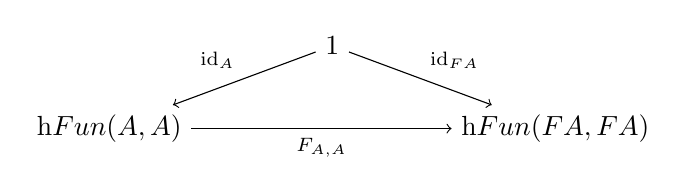
\begin{tikzpicture}[x=1.3em,y=1.3em]
  \node (1u) at (0,2.3) {$\mathbb{1}$};
  \node (l) at (-6.2,0) {$\mathrm{h}\Fun(A,A)$};
  \node (r) at (6.2,0) {$\mathrm{h}\Fun(FA,FA)$};
  \draw[->] (1u) -- node[above left]{$\scriptstyle\mathrm{id}_{A}$} (l);
  \draw[->] (1u) -- node[above right]{$\scriptstyle\mathrm{id}_{FA}$} (r);
  \draw[->] (l) -- node[below]{$\scriptstyle F_{A,A}$} (r);
\end{tikzpicture}
\par\vspace{0.8em}
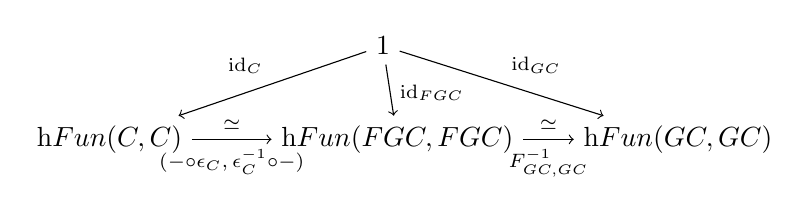
\begin{tikzpicture}[x=1.3em,y=1.3em]
  \node (1u) at (0,2.6) {$\mathbb{1}$};
  \node (l) at (-7.6,0) {$\mathrm{h}\Fun(C,C)$};
  \node (m) at (0.4,0) {$\mathrm{h}\Fun(FGC,FGC)$};
  \node (r) at (8.2,0) {$\mathrm{h}\Fun(GC,GC)$};
  \draw[->] (1u) -- node[above left]{$\scriptstyle\mathrm{id}_{C}$} (l);
  \draw[->] (1u) -- node[above right]{$\scriptstyle\mathrm{id}_{GC}$} (r);
  \draw[->] (1u) -- node[right,pos=0.55]{$\scriptstyle\mathrm{id}_{FGC}$} (m);
  \draw[->] (l) -- node[above]{$\scriptstyle\simeq$}
    node[below]{$\scriptstyle(-\circ\epsilon_{C},\,\epsilon_{C}^{-1}\circ-)$} (m);
  \draw[->] (m) -- node[above]{$\scriptstyle\simeq$}
    node[below]{$\scriptstyle F_{GC,GC}^{-1}$} (r);
\end{tikzpicture}
\end{center}

取而代之，映射 $G\colon\mathfrak{h}\mathcal{L}\rightsquigarrow\mathfrak{h}\mathcal{K}$
在诸\trHomotopyTwoCategory{}之间定义一个伪函子，这一概念我们现在予以回顾。

\begin{definition}\label{def:pseudofunctor}
介于 2-\trCategory{} $\mathcal{C}$ 与 $\mathcal{D}$ 之间的一个\textbf{伪函子}
$G\colon\mathcal{C}\rightsquigarrow\mathcal{D}$ 由如下数据给出：
\begin{itemize}
\item 对象上的一个映射 $\mathcal{C}\ni x\mapsto Gx\in\mathcal{D}$；
\item 对每一对 $x$、$y\in\mathcal{C}$，hom-\trCategory{}上的一个映射
$G_{x,y}\colon\mathcal{C}(x,y)\to\mathcal{D}(Gx,Gy)$；

\item 对每个 $x\in\mathcal{C}$，一个可逆 2-\trCell
\begin{center}
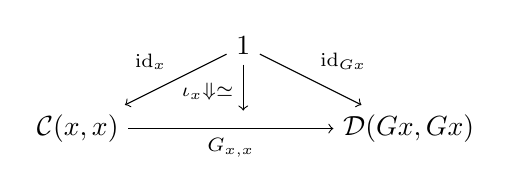
\begin{tikzpicture}[x=1.3em,y=1.3em]
  \node (1u) at (0,2.3) {$\mathbb{1}$};
  \node (l) at (-4.6,0) {$\mathcal{C}(x,x)$};
  \node (r) at (4.6,0) {$\mathcal{D}(Gx,Gx)$};
  \draw[->] (1u) -- node[above left]{$\scriptstyle\mathrm{id}_{x}$} (l);
  \draw[->] (1u) -- node[above right]{$\scriptstyle\mathrm{id}_{Gx}$} (r);
  \draw[->] (l) -- node[below]{$\scriptstyle G_{x,x}$} (r);
  \draw[->] (1u) -- node[left,pos=0.6]{$\scriptstyle\iota_{x}\Downarrow\simeq$} (0,0.5);
\end{tikzpicture}
\end{center}
它定义 $\mathcal{D}(Gx,Gx)$ 中的一个\trIsomorphism{}
$\iota_{x}\colon\mathrm{id}_{Gx}\cong G\,\mathrm{id}_{x}$\footnote{原书印作
「$G\,\mathrm{id}_{X}$」，末位系大写斜体 $X$；本条全句量词仅约束小写 $x$，且
其余诸处均作小写，应为排版笔误，此处径改。——译者注}；以及
\item 对每一三元组对象 $x$、$y$、$z\in\mathcal{C}$，一个自然同构
\begin{center}
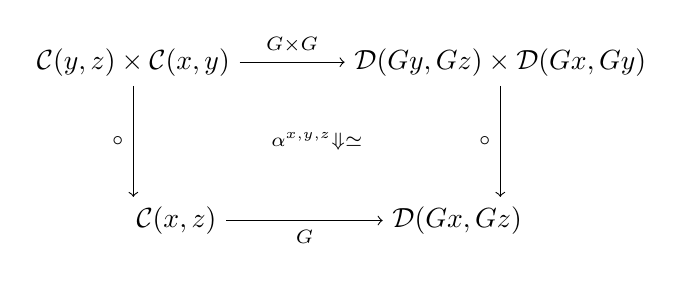
\begin{tikzpicture}[x=1.3em,y=1.3em]
  \node (tl) at (-4.8,2.2) {$\mathcal{C}(y,z)\times\mathcal{C}(x,y)$};
  \node (tr) at (5.4,2.2) {$\mathcal{D}(Gy,Gz)\times\mathcal{D}(Gx,Gy)$};
  \node (bl) at (-3.6,-2.2) {$\mathcal{C}(x,z)$};
  \node (br) at (4.2,-2.2) {$\mathcal{D}(Gx,Gz)$};
  \draw[->] (tl) -- node[above]{$\scriptstyle G{\times}G$} (tr);
  \draw[->] (bl) -- node[below]{$\scriptstyle G$} (br);
  \draw[->] (tl.south) -- node[left]{$\scriptstyle\circ$} (tl.south |- bl.north);
  \draw[->] (tr.south) -- node[left]{$\scriptstyle\circ$} (tr.south |- br.north);
  \node at (0.3,0) {$\scriptstyle\alpha^{x,y,z}\Downarrow\simeq$};
\end{tikzpicture}
\end{center}
满足由诸粘贴等式所编码的三条相干条件：
\begin{center}
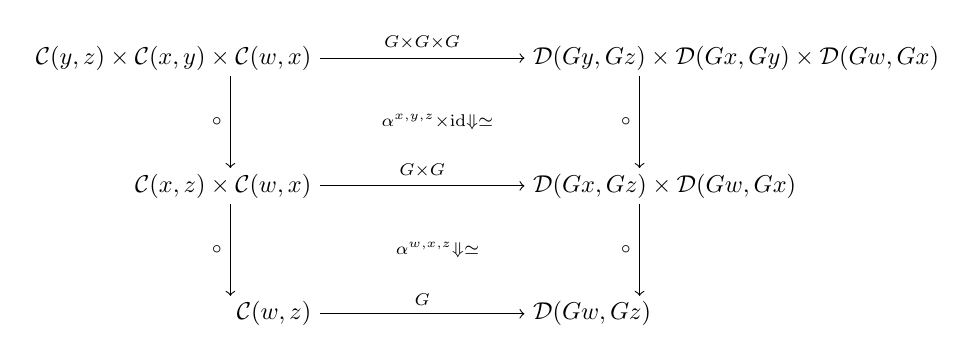
\begin{tikzpicture}[x=1.05em,y=1.05em,scale=0.88,transform shape]
  \node[anchor=east] (r1l) at (0,5) {$\mathcal{C}(y,z)\times\mathcal{C}(x,y)\times\mathcal{C}(w,x)$};
  \node[anchor=west] (r1r) at (8,5) {$\mathcal{D}(Gy,Gz)\times\mathcal{D}(Gx,Gy)\times\mathcal{D}(Gw,Gx)$};
  \node[anchor=east] (r2l) at (0,0) {$\mathcal{C}(x,z)\times\mathcal{C}(w,x)$};
  \node[anchor=west] (r2r) at (8,0) {$\mathcal{D}(Gx,Gz)\times\mathcal{D}(Gw,Gx)$};
  \node[anchor=east] (r3l) at (0,-5) {$\mathcal{C}(w,z)$};
  \node[anchor=west] (r3r) at (8,-5) {$\mathcal{D}(Gw,Gz)$};
  \draw[->] (r1l.east) -- node[above]{$\scriptstyle G{\times}G{\times}G$} (r1r.west);
  \draw[->] (r2l.east) -- node[above]{$\scriptstyle G{\times}G$} (r2r.west);
  \draw[->] (r3l.east) -- node[above]{$\scriptstyle G$} (r3r.west);
  \draw[->] (-3.5,4.3) -- node[left]{$\scriptstyle\circ$} (-3.5,0.7);
  \draw[->] (12.5,4.3) -- node[left]{$\scriptstyle\circ$} (12.5,0.7);
  \draw[->] (-3.5,-0.7) -- node[left]{$\scriptstyle\circ$} (-3.5,-4.3);
  \draw[->] (12.5,-0.7) -- node[left]{$\scriptstyle\circ$} (12.5,-4.3);
  \node at (4.6,2.5) {$\scriptstyle\alpha^{x,y,z}\times\mathrm{id}\Downarrow\simeq$};
  \node at (4.6,-2.5) {$\scriptstyle\alpha^{w,x,z}\Downarrow\simeq$};
\end{tikzpicture}
\par\vspace{0.5em}
\begin{tikzpicture}
  \draw[double,double distance=1.2pt] (0,0)--(0,0.75);
\end{tikzpicture}
\par\vspace{0.5em}
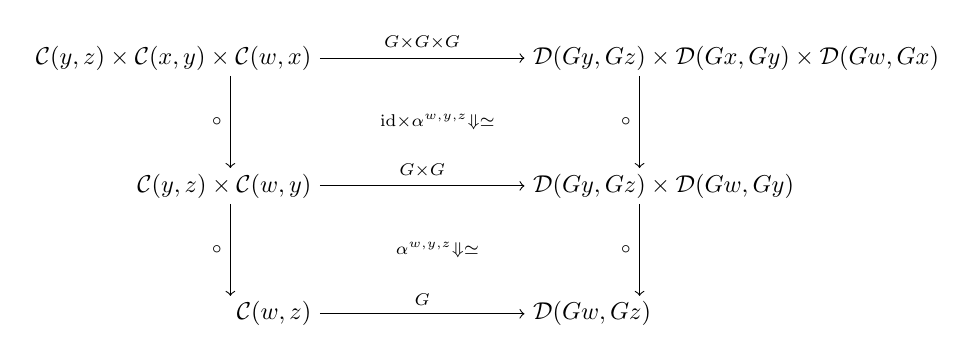
\begin{tikzpicture}[x=1.05em,y=1.05em,scale=0.88,transform shape]
  \node[anchor=east] (r1l) at (0,5) {$\mathcal{C}(y,z)\times\mathcal{C}(x,y)\times\mathcal{C}(w,x)$};
  \node[anchor=west] (r1r) at (8,5) {$\mathcal{D}(Gy,Gz)\times\mathcal{D}(Gx,Gy)\times\mathcal{D}(Gw,Gx)$};
  \node[anchor=east] (r2l) at (0,0) {$\mathcal{C}(y,z)\times\mathcal{C}(w,y)$};
  \node[anchor=west] (r2r) at (8,0) {$\mathcal{D}(Gy,Gz)\times\mathcal{D}(Gw,Gy)$};
  \node[anchor=east] (r3l) at (0,-5) {$\mathcal{C}(w,z)$};
  \node[anchor=west] (r3r) at (8,-5) {$\mathcal{D}(Gw,Gz)$};
  \draw[->] (r1l.east) -- node[above]{$\scriptstyle G{\times}G{\times}G$} (r1r.west);
  \draw[->] (r2l.east) -- node[above]{$\scriptstyle G{\times}G$} (r2r.west);
  \draw[->] (r3l.east) -- node[above]{$\scriptstyle G$} (r3r.west);
  \draw[->] (-3.5,4.3) -- node[left]{$\scriptstyle\circ$} (-3.5,0.7);
  \draw[->] (12.5,4.3) -- node[left]{$\scriptstyle\circ$} (12.5,0.7);
  \draw[->] (-3.5,-0.7) -- node[left]{$\scriptstyle\circ$} (-3.5,-4.3);
  \draw[->] (12.5,-0.7) -- node[left]{$\scriptstyle\circ$} (12.5,-4.3);
  \node at (4.6,2.5) {$\scriptstyle\mathrm{id}\times\alpha^{w,y,z}\Downarrow\simeq$};
  \node at (4.6,-2.5) {$\scriptstyle\alpha^{w,y,z}\Downarrow\simeq$};
\end{tikzpicture}
\end{center}
\begin{center}
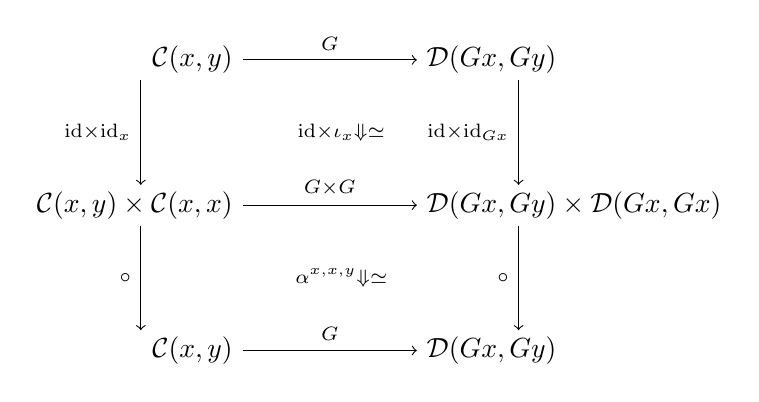
\begin{tikzpicture}[x=1.05em,y=1.05em]
  \node[anchor=east] (r1l) at (0,5) {$\mathcal{C}(x,y)$};
  \node[anchor=west] (r1r) at (6,5) {$\mathcal{D}(Gx,Gy)$};
  \node[anchor=east] (r2l) at (0,0) {$\mathcal{C}(x,y)\times\mathcal{C}(x,x)$};
  \node[anchor=west] (r2r) at (6,0) {$\mathcal{D}(Gx,Gy)\times\mathcal{D}(Gx,Gx)$};
  \node[anchor=east] (r3l) at (0,-5) {$\mathcal{C}(x,y)$};
  \node[anchor=west] (r3r) at (6,-5) {$\mathcal{D}(Gx,Gy)$};
  \draw[->] (r1l.east) -- node[above]{$\scriptstyle G$} (r1r.west);
  \draw[->] (r2l.east) -- node[above]{$\scriptstyle G{\times}G$} (r2r.west);
  \draw[->] (r3l.east) -- node[above]{$\scriptstyle G$} (r3r.west);
  \draw[->] (-3.5,4.3) -- node[left]{$\scriptstyle\mathrm{id}{\times}\mathrm{id}_{x}$} (-3.5,0.7);
  \draw[->] (9.5,4.3) -- node[left]{$\scriptstyle\mathrm{id}{\times}\mathrm{id}_{Gx}$} (9.5,0.7);
  \draw[->] (-3.5,-0.7) -- node[left]{$\scriptstyle\circ$} (-3.5,-4.3);
  \draw[->] (9.5,-0.7) -- node[left]{$\scriptstyle\circ$} (9.5,-4.3);
  \node at (3.4,2.5) {$\scriptstyle\mathrm{id}{\times}\iota_{x}\Downarrow\simeq$};
  \node at (3.4,-2.5) {$\scriptstyle\alpha^{x,x,y}\Downarrow\simeq$};
\end{tikzpicture}
\par\vspace{0.5em}
\begin{tikzpicture}
  \draw[double,double distance=1.2pt] (0,0)--(0,0.75);
\end{tikzpicture}
\par\vspace{0.5em}
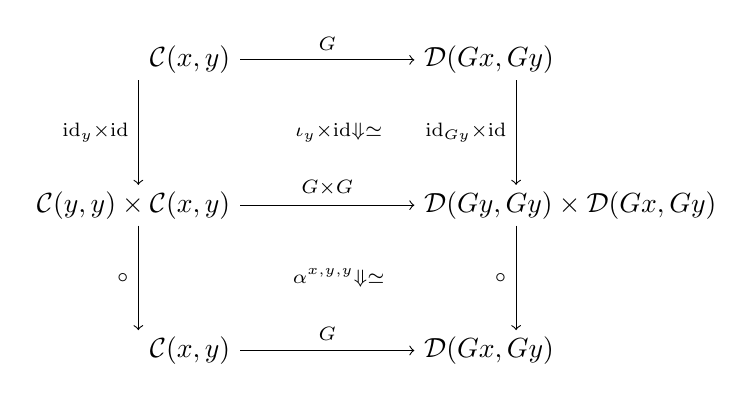
\begin{tikzpicture}[x=1.05em,y=1.05em]
  \node[anchor=east] (r1l) at (0,5) {$\mathcal{C}(x,y)$};
  \node[anchor=west] (r1r) at (6,5) {$\mathcal{D}(Gx,Gy)$};
  \node[anchor=east] (r2l) at (0,0) {$\mathcal{C}(y,y)\times\mathcal{C}(x,y)$};
  \node[anchor=west] (r2r) at (6,0) {$\mathcal{D}(Gy,Gy)\times\mathcal{D}(Gx,Gy)$};
  \node[anchor=east] (r3l) at (0,-5) {$\mathcal{C}(x,y)$};
  \node[anchor=west] (r3r) at (6,-5) {$\mathcal{D}(Gx,Gy)$};
  \draw[->] (r1l.east) -- node[above]{$\scriptstyle G$} (r1r.west);
  \draw[->] (r2l.east) -- node[above]{$\scriptstyle G{\times}G$} (r2r.west);
  \draw[->] (r3l.east) -- node[above]{$\scriptstyle G$} (r3r.west);
  \draw[->] (-3.5,4.3) -- node[left]{$\scriptstyle\mathrm{id}_{y}{\times}\mathrm{id}$} (-3.5,0.7);
  \draw[->] (9.5,4.3) -- node[left]{$\scriptstyle\mathrm{id}_{Gy}{\times}\mathrm{id}$} (9.5,0.7);
  \draw[->] (-3.5,-0.7) -- node[left]{$\scriptstyle\circ$} (-3.5,-4.3);
  \draw[->] (9.5,-0.7) -- node[left]{$\scriptstyle\circ$} (9.5,-4.3);
  \node at (3.4,2.5) {$\scriptstyle\iota_{y}{\times}\mathrm{id}\Downarrow\simeq$};
  \node at (3.4,-2.5) {$\scriptstyle\alpha^{x,y,y}\Downarrow\simeq$};
\end{tikzpicture}
\end{center}
其中这两个后者的复合均等于单位 2-\trCell{}
$\mathrm{id}_{G_{x,y}}$。
\end{itemize}
\end{definition}

一个\textbf{2-\trFunctor}是这样的伪函子：其中单位胞腔与复合胞腔 $\iota$ 与
$\alpha$ 均为恒同。2-\trFunctor{}之间的 2-自然变换（见附录 B 中的%
\cref{def:two-natural-transformation}）这一概念，
同样地推广为伪函子之间的伪自然变换。

\begin{definition}\label{def:pseudonatural-transformation}
对任意一对 2-\trCategory{} $\mathcal{C}$ 与 $\mathcal{D}$ 以及平行的伪函子
$F$、$G\colon\mathcal{C}\rightsquigarrow\mathcal{D}$，一个\textbf{伪自然变换}
$\phi\colon F\Rrightarrow G$ 由如下数据给出：
\begin{itemize}
\item 对每个对象 $x\in\mathcal{C}$，一个 1-\trCell{}
$\phi_{x}\colon Fx\to Gx\in\mathcal{D}$；并且
\item 对每个 1-\trCell{} $f\colon x\to y\in\mathcal{C}$，$\mathcal{D}$ 中的一个
可逆 2-\trCell
\begin{center}
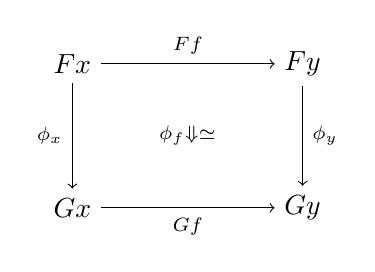
\begin{tikzpicture}[x=1.3em,y=1.3em]
  \node (tl) at (-3.2,2) {$Fx$};
  \node (tr) at (3.2,2) {$Fy$};
  \node (bl) at (-3.2,-2) {$Gx$};
  \node (br) at (3.2,-2) {$Gy$};
  \draw[->] (tl) -- node[above]{$\scriptstyle Ff$} (tr);
  \draw[->] (bl) -- node[below]{$\scriptstyle Gf$} (br);
  \draw[->] (tl) -- node[left]{$\scriptstyle\phi_{x}$} (bl);
  \draw[->] (tr) -- node[right]{$\scriptstyle\phi_{y}$} (br);
  \node at (0,0) {$\scriptstyle\phi_{f}\Downarrow\simeq$};
\end{tikzpicture}
\end{center}
使得这批数据
\item 是自然的，其意义为：对 $\mathcal{C}$ 中的每个 2-\trCell{}
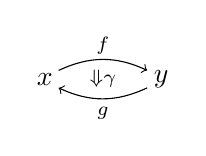
\begin{tikzpicture}[x=1em,y=0.9em,baseline=-0.5em]
  \node (x) at (0,0) {$x$};
  \node (y) at (4.2,0) {$y$};
  \draw[->] (0.5,0.35) to[bend left=25] (3.7,0.35);
  \node at (2.1,1.35) {$\scriptstyle f$};
  \draw[->] (3.7,-0.35) to[bend left=25] (0.5,-0.35);
  \node at (2.1,-1.35) {$\scriptstyle g$};
  \node at (2.1,0) {$\scriptstyle\Downarrow\gamma$};
\end{tikzpicture}
（$\mathcal{C}$ 中），粘贴复合相等
\begin{center}
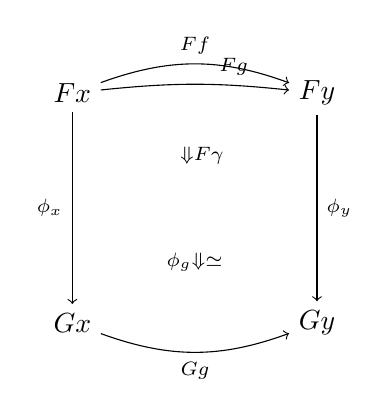
\begin{tikzpicture}[x=1.3em,y=1.3em]
  \node (tl) at (-3.4,3.2) {$Fx$};
  \node (tr) at (3.4,3.2) {$Fy$};
  \node (bl) at (-3.4,-3.2) {$Gx$};
  \node (br) at (3.4,-3.2) {$Gy$};
  \draw[->] (tl) to[bend left=20] node[above]{$\scriptstyle Ff$} (tr);
  \draw[->] (tl) to[bend left=6] node[above,pos=0.72]{$\scriptstyle Fg$} (tr);
  \node at (0.2,1.45) {$\scriptstyle\Downarrow F\gamma$};
  \draw[->] (tl) -- node[left]{$\scriptstyle\phi_{x}$} (bl);
  \draw[->] (tr) -- node[right]{$\scriptstyle\phi_{y}$} (br);
  \node at (0,-1.5) {$\scriptstyle\phi_{g}\Downarrow\simeq$};
  \draw[->] (bl) to[bend right=20] node[below]{$\scriptstyle Gg$} (br);
\end{tikzpicture}
\quad$=$\quad
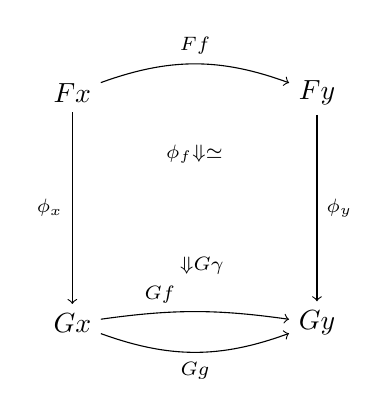
\begin{tikzpicture}[x=1.3em,y=1.3em]
  \node (tl) at (-3.4,3.2) {$Fx$};
  \node (tr) at (3.4,3.2) {$Fy$};
  \node (bl) at (-3.4,-3.2) {$Gx$};
  \node (br) at (3.4,-3.2) {$Gy$};
  \draw[->] (tl) to[bend left=20] node[above]{$\scriptstyle Ff$} (tr);
  \node at (0,1.5) {$\scriptstyle\phi_{f}\Downarrow\simeq$};
  \draw[->] (tl) -- node[left]{$\scriptstyle\phi_{x}$} (bl);
  \draw[->] (tr) -- node[right]{$\scriptstyle\phi_{y}$} (br);
  \draw[->] (bl) to[bend left=8] node[above,pos=0.3]{$\scriptstyle Gf$} (br);
  \node at (0.2,-1.6) {$\scriptstyle\Downarrow G\gamma$};
  \draw[->] (bl) to[bend right=20] node[below]{$\scriptstyle Gg$} (br);
\end{tikzpicture}
\end{center}
；以及
\item 尊重由诸伪函子指定的复合约束与单位约束：
\begin{center}
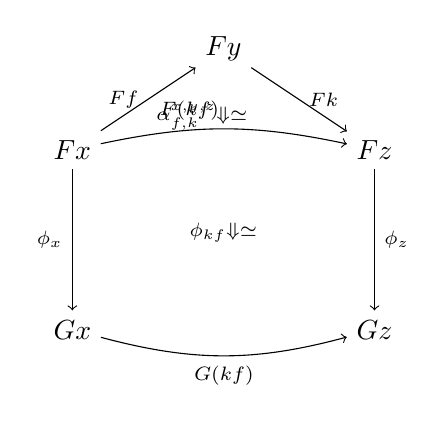
\begin{tikzpicture}[x=1.3em,y=1.3em]
  \node (fx) at (-4.2,0.6) {$Fx$};
  \node (fy) at (0,3.4) {$Fy$};
  \node (fz) at (4.2,0.6) {$Fz$};
  \node (gx) at (-4.2,-4.4) {$Gx$};
  \node (gz) at (4.2,-4.4) {$Gz$};
  \draw[->] (fx) -- node[above,left]{$\scriptstyle Ff$} (fy);
  \draw[->] (fy) -- node[above,right]{$\scriptstyle Fk$} (fz);
  \node at (-0.6,1.5) {$\scriptstyle\alpha^{x,y,z}_{f,k}\Downarrow\simeq$};
  \draw[->] (fx) to[bend left=12] node[above,pos=0.35]{$\scriptstyle F(kf)$} (fz);
  \node at (0,-1.7) {$\scriptstyle\phi_{kf}\Downarrow\simeq$};
  \draw[->] (fx) -- node[left]{$\scriptstyle\phi_{x}$} (gx);
  \draw[->] (fz) -- node[right]{$\scriptstyle\phi_{z}$} (gz);
  \draw[->] (gx) to[bend right=15] node[below]{$\scriptstyle G(kf)$} (gz);
\end{tikzpicture}
\quad$=$\quad
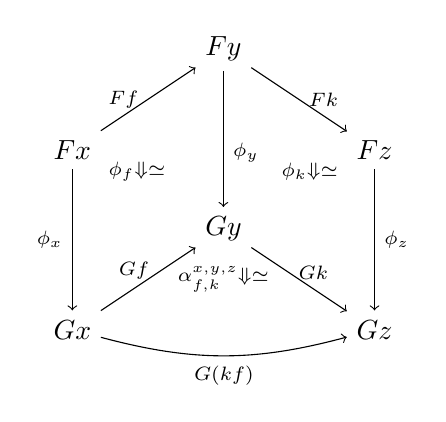
\begin{tikzpicture}[x=1.3em,y=1.3em]
  \node (fx) at (-4.2,0.6) {$Fx$};
  \node (fy) at (0,3.4) {$Fy$};
  \node (fz) at (4.2,0.6) {$Fz$};
  \node (gx) at (-4.2,-4.4) {$Gx$};
  \node (gy) at (0,-1.6) {$Gy$};
  \node (gz) at (4.2,-4.4) {$Gz$};
  \draw[->] (fx) -- node[above,left]{$\scriptstyle Ff$} (fy);
  \draw[->] (fy) -- node[above,right]{$\scriptstyle Fk$} (fz);
  \draw[->] (fx) -- node[left]{$\scriptstyle\phi_{x}$} (gx);
  \draw[->] (fy) -- node[right,pos=0.6]{$\scriptstyle\phi_{y}$} (gy);
  \draw[->] (fz) -- node[right]{$\scriptstyle\phi_{z}$} (gz);
  \node at (-2.4,0) {$\scriptstyle\phi_{f}\Downarrow\simeq$};
  \node at (2.4,0) {$\scriptstyle\phi_{k}\Downarrow\simeq$};
  \draw[->] (gx) -- node[above,pos=0.35]{$\scriptstyle Gf$} (gy);
  \draw[->] (gy) -- node[above,pos=0.65]{$\scriptstyle Gk$} (gz);
  \node at (0,-3.0) {$\scriptstyle\alpha^{x,y,z}_{f,k}\Downarrow\simeq$};
  \draw[->] (gx) to[bend right=15] node[below]{$\scriptstyle G(kf)$} (gz);
\end{tikzpicture}
\end{center}
\par 以及
\begin{center}
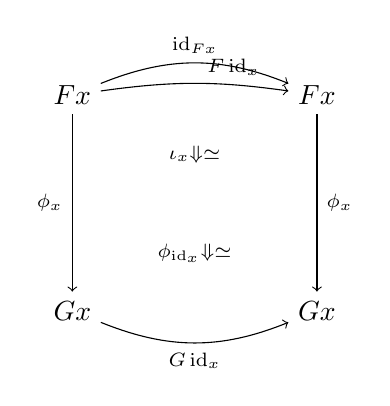
\begin{tikzpicture}[x=1.3em,y=1.3em]
  \node (tl) at (-3.4,3.0) {$Fx$};
  \node (tr) at (3.4,3.0) {$Fx$};
  \node (bl) at (-3.4,-3.0) {$Gx$};
  \node (br) at (3.4,-3.0) {$Gx$};
  \draw[->] (tl) to[bend left=22] node[above]{$\scriptstyle\mathrm{id}_{Fx}$} (tr);
  \draw[->] (tl) to[bend left=8] node[above,pos=0.72]{$\scriptstyle F\,\mathrm{id}_{x}$} (tr);
  \node at (0,1.35) {$\scriptstyle\iota_{x}\Downarrow\simeq$};
  \draw[->] (tl) -- node[left]{$\scriptstyle\phi_{x}$} (bl);
  \draw[->] (tr) -- node[right]{$\scriptstyle\phi_{x}$} (br);
  \node at (0,-1.4) {$\scriptstyle\phi_{\mathrm{id}_{x}}\Downarrow\simeq$};
  \draw[->] (bl) to[bend right=22] node[below]{$\scriptstyle G\,\mathrm{id}_{x}$} (br);
\end{tikzpicture}
\quad$=$\quad
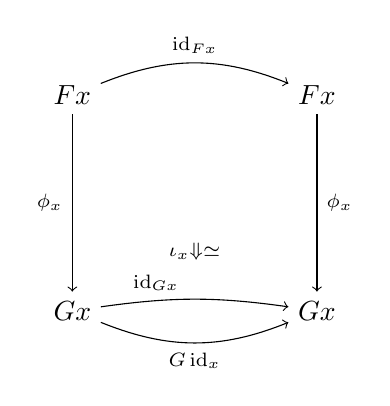
\begin{tikzpicture}[x=1.3em,y=1.3em]
  \node (tl) at (-3.4,3.0) {$Fx$};
  \node (tr) at (3.4,3.0) {$Fx$};
  \node (bl) at (-3.4,-3.0) {$Gx$};
  \node (br) at (3.4,-3.0) {$Gx$};
  \draw[->] (tl) to[bend left=22] node[above]{$\scriptstyle\mathrm{id}_{Fx}$} (tr);
  \draw[->] (tl) -- node[left]{$\scriptstyle\phi_{x}$} (bl);
  \draw[->] (tr) -- node[right]{$\scriptstyle\phi_{x}$} (br);
  \draw[->] (bl) to[bend left=8] node[above,pos=0.28]{$\scriptstyle\mathrm{id}_{Gx}$} (br);
  \node at (0,-1.35) {$\scriptstyle\iota_{x}\Downarrow\simeq$};
  \draw[->] (bl) to[bend right=22] node[below]{$\scriptstyle G\,\mathrm{id}_{x}$} (br);
\end{tikzpicture}
\footnote{原书此图之中部 2-胞腔印作「$\iota_{y}\Downarrow\simeq$」，然图中诸对象
皆为 $x$，按单位胞腔语义系 $G$ 在 $x$ 处之单位 2-胞腔 $\iota_{x}$，此处径改。——译者注}
\end{center}
\end{itemize}
\end{definition}

伪函子浮现的一个语境，是作为定义\trBiequivalence{}的 2-\trFunctor{}之逆。
以此方式浮现的伪函子本身是\textbf{双等价的}：依等价意义于对象上为满，并且在
hom-\trCategory{}上定义\trLocalEquivalence。这些\trFunctor{}是逆，其意义为：
在各复合与诸恒同之间存在\textbf{伪自然等价}——即逐分量地成为\trEquivalence{}的
伪自然变换（另一刻画见\cref{ex:pseudonatural-equivalence-characterization}）。
总体而言，这批数据定义了 2-\trCategory{}%
在适合于\trBicategory{}理论之意义上的一个\trEquivalence：

\begin{proposition}\label{prop:pseudoinverse-2-functor}
若 $F\colon\mathcal{C}\to\mathcal{D}$ 是 2-\trCategory{} $\mathcal{C}$ 与
$\mathcal{D}$ 之间的一个 2-\trFunctor{}兼\trBiequivalence，则存在一个伪函子
$G\colon\mathcal{D}\rightsquigarrow\mathcal{C}$，它也是\trBiequivalence，并且在
下述意义下是 $F$ 的一个\emph{伪逆}（pseudoinverse）：存在伪自然等价
$\mathrm{id}_{\mathcal{C}}\Rrightarrow GF$ 与
$FG\Rrightarrow\mathrm{id}_{\mathcal{D}}$。
\end{proposition}

\begin{proof}
\cref{ex:derive-prop-1043}。
\end{proof}

命题 10.4.3 描述了\trBicategory{}理论中的一个经典结果，Johnson 与 Yau 称之为%
「\trBicategory{} Whitehead 定理」[59, 7.4.1]，所以我们心安理得地把它的证明留给练习（亦见%
\cref{prop:quasi-pseudoinverse}）。

请回忆定义 1.2.1：一个\trInfinityCosmos{}除其他外，是一个在诸\trQuasiCategory{}之%
\trCartesianClosed\trCategory{}中富集的\trCategory；而一支\trCosmologicalFunctor{}除其他外，
是诸拟范畴富集\trCategory{}之间的一个富集\trFunctor{}（见 A.2 节）。
为定义一个拟范畴富集伪函子，我们需要把由\trQuasiCategory{}与\trFunctor{}构成的
1-\trCategory{}扩张为一座 2-\trCategory，从而可以利用它的 2-\trCell{}来编码单位
相干与复合相干。幸运的是，我们手头正有这样一座 2-\trCategory：\trQuasiCategory{}的%
\trHomotopyTwoCategory{} $\mathfrak{h}\QCat$。由命题 1.4.5，这座由拟范畴、其间的%
\trFunctor{}以及其间的\trNaturalTransformation{}构成的 2-\trCategory{}是%
\trCartesianClosed{}，于是我们在这些 2-\trCell{}上拥有良态的\trCartesianProduct{}与
转置运算。

$\mathfrak{h}\QCat$ 这座 2-\trCategory{}中的额外维数，使我们能够如下定义拟范畴
富集伪函子：

\begin{definition}\label{def:quasi-pseudofunctor}
对诸拟范畴富集\trCategory{} $\mathcal{K}$ 与 $\mathcal{L}$，一个\textbf{拟范畴
富集伪函子} $G\colon\mathcal{K}\rightsquigarrow\mathcal{L}$——简称\textbf{拟伪函子}
——由如下数据给出：
\begin{itemize}
\item 对象上的一个映射 $\mathcal{K}\ni x\mapsto Gx\in\mathcal{L}$；
\item 对每一对 $x$、$y\in\mathcal{K}$，hom-\trQuasiCategory{}之间的一个\trFunctor{}
$G_{x,y}\colon\mathcal{K}(x,y)\to\mathcal{L}(Gx,Gy)$；
\item 对每个 $x\in\mathcal{K}$，在诸\trQuasiCategory{}的\trHomotopyTwoCategory{}中的一个
可逆 2-\trCell
\begin{center}
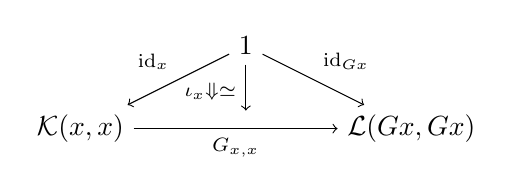
\begin{tikzpicture}[x=1.3em,y=1.3em]
  \node (1u) at (0,2.3) {$\mathbb{1}$};
  \node (l) at (-4.6,0) {$\mathcal{K}(x,x)$};
  \node (r) at (4.6,0) {$\mathcal{L}(Gx,Gx)$};
  \draw[->] (1u) -- node[above left]{$\scriptstyle\mathrm{id}_{x}$} (l);
  \draw[->] (1u) -- node[above right]{$\scriptstyle\mathrm{id}_{Gx}$} (r);
  \draw[->] (l) -- node[below]{$\scriptstyle G_{x,x}$} (r);
  \draw[->] (1u) -- node[left,pos=0.6]{$\scriptstyle\iota_{x}\Downarrow\simeq$} (0,0.5);
\end{tikzpicture}
\end{center}
\item 对每一三元组对象 $x$、$y$、$z\in\mathcal{K}$，在诸拟范畴的%
\trHomotopyTwoCategory{}中的一个可逆 2-\trCell
\begin{center}
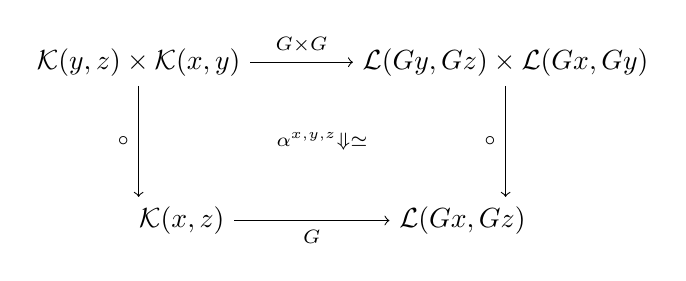
\begin{tikzpicture}[x=1.3em,y=1.3em]
  \node (tl) at (-4.8,2.2) {$\mathcal{K}(y,z)\times\mathcal{K}(x,y)$};
  \node (tr) at (5.4,2.2) {$\mathcal{L}(Gy,Gz)\times\mathcal{L}(Gx,Gy)$};
  \node (bl) at (-3.6,-2.2) {$\mathcal{K}(x,z)$};
  \node (br) at (4.2,-2.2) {$\mathcal{L}(Gx,Gz)$};
  \draw[->] (tl) -- node[above]{$\scriptstyle G{\times}G$} (tr);
  \draw[->] (bl) -- node[below]{$\scriptstyle G$} (br);
  \draw[->] (tl.south) -- node[left]{$\scriptstyle\circ$} (tl.south |- bl.north);
  \draw[->] (tr.south) -- node[left]{$\scriptstyle\circ$} (tr.south |- br.north);
  \node at (0.3,0) {$\scriptstyle\alpha^{x,y,z}\Downarrow\simeq$};
\end{tikzpicture}
\end{center}

满足由诸粘贴等式所编码的三条相干条件：
\begin{rveq}\label{eq:quasi-pseudofunctor-pasting}
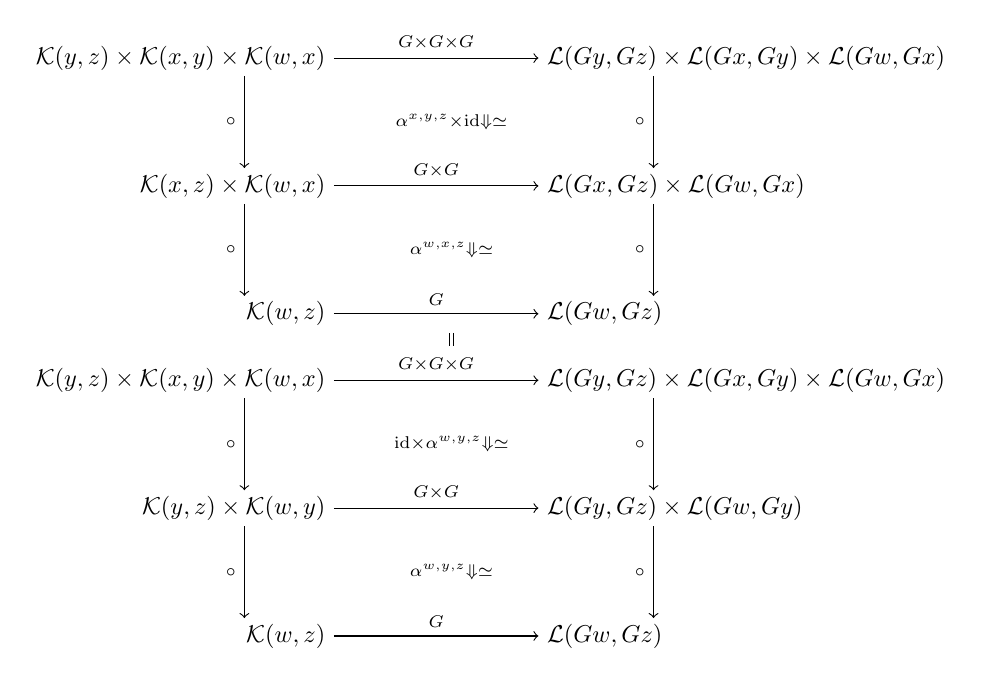
\begin{tikzpicture}[x=1.05em,y=1.05em,scale=0.88,transform shape]
  \node[anchor=east] (r1l) at (0,5) {$\mathcal{K}(y,z)\times\mathcal{K}(x,y)\times\mathcal{K}(w,x)$};
  \node[anchor=west] (r1r) at (8,5) {$\mathcal{L}(Gy,Gz)\times\mathcal{L}(Gx,Gy)\times\mathcal{L}(Gw,Gx)$};
  \node[anchor=east] (r2l) at (0,0) {$\mathcal{K}(x,z)\times\mathcal{K}(w,x)$};
  \node[anchor=west] (r2r) at (8,0) {$\mathcal{L}(Gx,Gz)\times\mathcal{L}(Gw,Gx)$};
  \node[anchor=east] (r3l) at (0,-5) {$\mathcal{K}(w,z)$};
  \node[anchor=west] (r3r) at (8,-5) {$\mathcal{L}(Gw,Gz)$};
  \draw[->] (r1l.east) -- node[above]{$\scriptstyle G{\times}G{\times}G$} (r1r.west);
  \draw[->] (r2l.east) -- node[above]{$\scriptstyle G{\times}G$} (r2r.west);
  \draw[->] (r3l.east) -- node[above]{$\scriptstyle G$} (r3r.west);
  \draw[->] (-3.5,4.3) -- node[left]{$\scriptstyle\circ$} (-3.5,0.7);
  \draw[->] (12.5,4.3) -- node[left]{$\scriptstyle\circ$} (12.5,0.7);
  \draw[->] (-3.5,-0.7) -- node[left]{$\scriptstyle\circ$} (-3.5,-4.3);
  \draw[->] (12.5,-0.7) -- node[left]{$\scriptstyle\circ$} (12.5,-4.3);
  \node at (4.6,2.5) {$\scriptstyle\alpha^{x,y,z}\times\mathrm{id}\Downarrow\simeq$};
  \node at (4.6,-2.5) {$\scriptstyle\alpha^{w,x,z}\Downarrow\simeq$};
  \draw[double,double distance=1.2pt] (4.6,-5.75) -- (4.6,-6.25);
  \node[anchor=east] (r1l) at (0,-7.6) {$\mathcal{K}(y,z)\times\mathcal{K}(x,y)\times\mathcal{K}(w,x)$};
  \node[anchor=west] (r1r) at (8,-7.6) {$\mathcal{L}(Gy,Gz)\times\mathcal{L}(Gx,Gy)\times\mathcal{L}(Gw,Gx)$};
  \node[anchor=east] (r2l) at (0,-12.6) {$\mathcal{K}(y,z)\times\mathcal{K}(w,y)$};
  \node[anchor=west] (r2r) at (8,-12.6) {$\mathcal{L}(Gy,Gz)\times\mathcal{L}(Gw,Gy)$};
  \node[anchor=east] (r3l) at (0,-17.6) {$\mathcal{K}(w,z)$};
  \node[anchor=west] (r3r) at (8,-17.6) {$\mathcal{L}(Gw,Gz)$};
  \draw[->] (r1l.east) -- node[above]{$\scriptstyle G{\times}G{\times}G$} (r1r.west);
  \draw[->] (r2l.east) -- node[above]{$\scriptstyle G{\times}G$} (r2r.west);
  \draw[->] (r3l.east) -- node[above]{$\scriptstyle G$} (r3r.west);
  \draw[->] (-3.5,-8.3) -- node[left]{$\scriptstyle\circ$} (-3.5,-11.9);
  \draw[->] (12.5,-8.3) -- node[left]{$\scriptstyle\circ$} (12.5,-11.9);
  \draw[->] (-3.5,-13.3) -- node[left]{$\scriptstyle\circ$} (-3.5,-16.9);
  \draw[->] (12.5,-13.3) -- node[left]{$\scriptstyle\circ$} (12.5,-16.9);
  \node at (4.6,-10.1) {$\scriptstyle\mathrm{id}{\times}\alpha^{w,y,z}\Downarrow\simeq$};
  \node at (4.6,-15.1) {$\scriptstyle\alpha^{w,y,z}\Downarrow\simeq$};
\end{tikzpicture}
\end{rveq}
\begin{center}
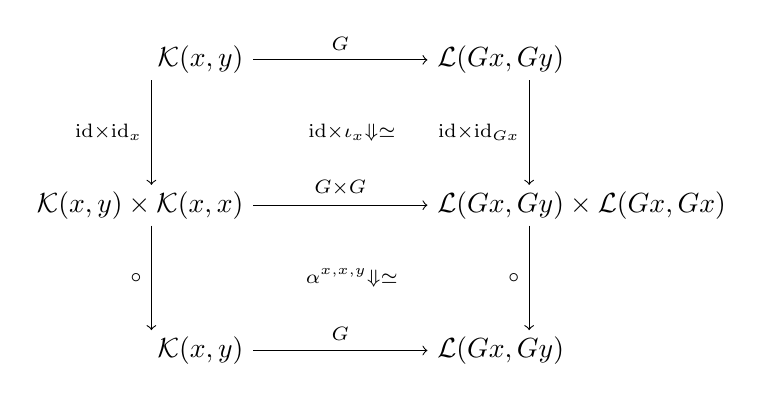
\begin{tikzpicture}[x=1.05em,y=1.05em]
  \node[anchor=east] (r1l) at (0,5) {$\mathcal{K}(x,y)$};
  \node[anchor=west] (r1r) at (6,5) {$\mathcal{L}(Gx,Gy)$};
  \node[anchor=east] (r2l) at (0,0) {$\mathcal{K}(x,y)\times\mathcal{K}(x,x)$};
  \node[anchor=west] (r2r) at (6,0) {$\mathcal{L}(Gx,Gy)\times\mathcal{L}(Gx,Gx)$};
  \node[anchor=east] (r3l) at (0,-5) {$\mathcal{K}(x,y)$};
  \node[anchor=west] (r3r) at (6,-5) {$\mathcal{L}(Gx,Gy)$};
  \draw[->] (r1l.east) -- node[above]{$\scriptstyle G$} (r1r.west);
  \draw[->] (r2l.east) -- node[above]{$\scriptstyle G{\times}G$} (r2r.west);
  \draw[->] (r3l.east) -- node[above]{$\scriptstyle G$} (r3r.west);
  \draw[->] (-3.5,4.3) -- node[left]{$\scriptstyle\mathrm{id}{\times}\mathrm{id}_{x}$} (-3.5,0.7);
  \draw[->] (9.5,4.3) -- node[left]{$\scriptstyle\mathrm{id}{\times}\mathrm{id}_{Gx}$} (9.5,0.7);
  \draw[->] (-3.5,-0.7) -- node[left]{$\scriptstyle\circ$} (-3.5,-4.3);
  \draw[->] (9.5,-0.7) -- node[left]{$\scriptstyle\circ$} (9.5,-4.3);
  \node at (3.4,2.5) {$\scriptstyle\mathrm{id}{\times}\iota_{x}\Downarrow\simeq$};
  \node at (3.4,-2.5) {$\scriptstyle\alpha^{x,x,y}\Downarrow\simeq$};
\end{tikzpicture}
\par\vspace{0.4em}
$=$
\par\vspace{0.4em}
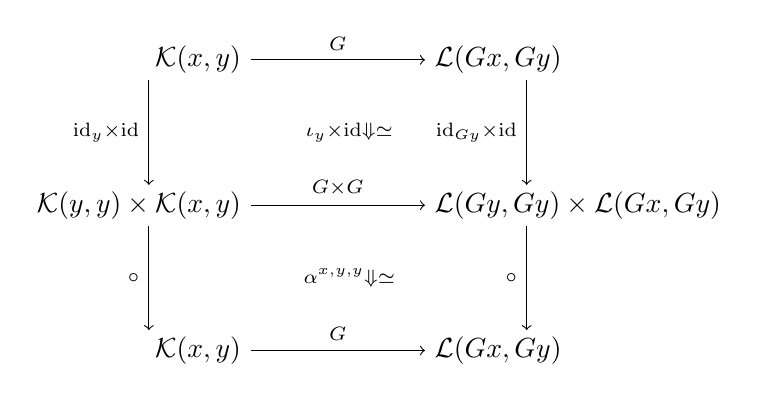
\begin{tikzpicture}[x=1.05em,y=1.05em]
  \node[anchor=east] (r1l) at (0,5) {$\mathcal{K}(x,y)$};
  \node[anchor=west] (r1r) at (6,5) {$\mathcal{L}(Gx,Gy)$};
  \node[anchor=east] (r2l) at (0,0) {$\mathcal{K}(y,y)\times\mathcal{K}(x,y)$};
  \node[anchor=west] (r2r) at (6,0) {$\mathcal{L}(Gy,Gy)\times\mathcal{L}(Gx,Gy)$};
  \node[anchor=east] (r3l) at (0,-5) {$\mathcal{K}(x,y)$};
  \node[anchor=west] (r3r) at (6,-5) {$\mathcal{L}(Gx,Gy)$};
  \draw[->] (r1l.east) -- node[above]{$\scriptstyle G$} (r1r.west);
  \draw[->] (r2l.east) -- node[above]{$\scriptstyle G{\times}G$} (r2r.west);
  \draw[->] (r3l.east) -- node[above]{$\scriptstyle G$} (r3r.west);
  \draw[->] (-3.5,4.3) -- node[left]{$\scriptstyle\mathrm{id}_{y}{\times}\mathrm{id}$} (-3.5,0.7);
  \draw[->] (9.5,4.3) -- node[left]{$\scriptstyle\mathrm{id}_{Gy}{\times}\mathrm{id}$} (9.5,0.7);
  \draw[->] (-3.5,-0.7) -- node[left]{$\scriptstyle\circ$} (-3.5,-4.3);
  \draw[->] (9.5,-0.7) -- node[left]{$\scriptstyle\circ$} (9.5,-4.3);
  \node at (3.4,2.5) {$\scriptstyle\iota_{y}{\times}\mathrm{id}\Downarrow\simeq$};
  \node at (3.4,-2.5) {$\scriptstyle\alpha^{x,y,y}\Downarrow\simeq$};
\end{tikzpicture}
\end{center}
其中这两个后者的复合均等于单位 2-\trCell{} $\mathrm{id}_{G_{x,y}}$。
\end{itemize}
\end{definition}

\begin{remark}\label{rem:terminal-qcat-notation}
为强调定义 10.4.1 与定义 10.4.4 之间的类似性，我们以 $\mathbb{1}$ 记%
\trTerminal{}\trQuasiCategory——它同时是终\trCategory{}的\trNerve；在别处，我们以 $1$ 记
一般\trInfinityCosmos{}中的\trTerminal{}∞-\trCategory。对拟范畴富集\trCategory{}中的
任意一对对象 $a$、$b\in\mathcal{L}$，有
\begin{equation*}
\Fun(\mathbb{1},\mathcal{L}(a,b))\cong\mathcal{L}(a,b),
\end{equation*}
从而 $\mathrm{h}\Fun(\mathbb{1},\mathcal{L}(a,b))\simeq\mathrm{h}\mathcal{L}(a,b)$。
于是，诸拟范畴之\trHomotopyTwoCategory{} $\mathfrak{h}\QCat$ 中以 $\mathbb{1}$ 为
定义域、以 $\mathcal{L}(a,b)$ 为余定义域的 2-\trCell{}，对应于 $\mathcal{L}$ 之%
\trHomotopyTwoCategory{}中从 $a$ 到 $b$ 的 2-\trCell{}——后者的定义与定义 1.4.1
所给者完全一致。
特别地，可逆 2-\trCell{} $\iota_{x}$ 之数据不多不少，恰是 $\mathcal{L}$ 之%
\trHomotopyTwoCategory{}中的一个可逆 2-\trCell
\begin{center}
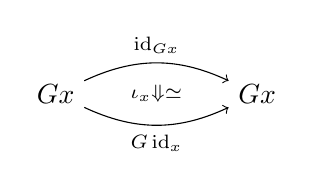
\begin{tikzpicture}[x=1.3em,y=1.3em]
  \node (l) at (-2.8,0) {$Gx$};
  \node (r) at (2.8,0) {$Gx$};
  \draw[->] (l) to[bend left=25] node[above]{$\scriptstyle\mathrm{id}_{Gx}$} (r);
  \draw[->] (l) to[bend right=25] node[below]{$\scriptstyle G\,\mathrm{id}_{x}$} (r);
  \node at (0,0) {$\scriptstyle\iota_{x}\Downarrow\simeq$};
\end{tikzpicture}
\end{center}
\end{remark}

定义 10.4.4 所引入的「拟伪函子」概念，应当被看作某个 $(\infty,2)$-范畴论概念的
2-范畴式截断，其意义如下：

\begin{digression}[拟伪函子作为 $(\infty,2)$-函子]\label{dig:quasi-pseudofunctor-infinity-2-functor}
诸拟范畴富集\trCategory{}之间的拟范畴富集\trFunctor{}可以被理解为「%
$(\infty,2)$-\trCategory{}之\trFunctor」。确实，单纯富集\trCategory{}之\trCategory{}带有
一个\trModelStructure，它呈现 $(\infty,2)$-\trCategory{}的 $(\infty,1)$-\trCategory，
其中诸\trFibrant{}对象恰是诸拟范畴富集\trCategory{} [79, 0.0.4]。然而，这一%
\trCategory{}中的诸\trFibrant{}对象未必是\trCofibrant{}的。\trCofibrant{}对象是由
Dwyer 与 Kan 最先定义的\trSimplicialComputad{} [37, 4.5]。
所以，要把一个从 $\mathcal{K}$ 到 $\mathcal{L}$ 的一般的 $(\infty,2)$-范畴论%
\trFunctor{}建模为拟范畴富集\trFunctor，必须先把 $\mathcal{K}$ 替换为一个弱等价的%
\trSimplicialComputad。
\end{digression}

这解释了为何一支\trCosmologicalBiequivalence{}之逆未必是一个严格的%
\trSimplicialFunctor，而是某种更弱的东西。列举拟范畴富集伪函子之数据的那些
2-\trCell{}相干，可以理解为「$(\infty,2)$-\trCategory{}之\trFunctor」的更高相干的
一个截断——正如诸\trQuasiCategory{}之\trHomotopyTwoCategory{}是拟范畴的拟范畴富集%
\trCategory{}的一个截断。既然本文的一个主题是：∞-范畴论的许多内容可以在截断后的%
\trHomotopyTwoCategory{}中、而非完整的 $(\infty,2)$-\trCategory{}中展开，我们便
不愿把\trCosmologicalBiequivalence{}之逆的更高相干作为定义 10.4.4 的一部分来列举。

\begin{definition}\label{def:quasi-biequivalence}
余定义域 $\mathcal{L}$ 为一个\trInfinityCosmos{}的拟伪函子
$G\colon\mathcal{K}\rightsquigarrow\mathcal{L}$，当它满足下列条件时是一个%
\textbf{\trBiequivalence}：
\begin{enumerate}[label=(\roman*)]
\item 依等价意义于对象上为满：若对一切 $a\in\mathcal{L}$ 都存在 $x\in\mathcal{K}$
使得 $Gx\simeq a$；并且
\footnote{原书印作「so that $Fx\simeq a$」，按定义头（拟伪函子记作 $G$）与本条
(ii) 之 $G_{x,y}$ 应为 $Gx$ 之误，此处径改。——译者注}
\item 诸\trQuasiCategory{}的一个\trLocalEquivalence：若对每一对 $x$、$y\in\mathcal{K}$，映射
\begin{equation*}
\mathcal{K}(x,y)\overset{G_{x,y}}{\xrightarrow{\ \sim\ }}\mathcal{L}(Gx,Gy)
\end{equation*}
是诸\trQuasiCategory{}之间的一个\trEquivalence。
\end{enumerate}
\end{definition}
\begin{remark}\label{rem:quasi-biequivalence-cosmos-codomain}
我们发现，在定义 10.4.8 中假定 $\mathcal{L}$ 是一个\trInfinityCosmos{}是方便的，
因为这使得我们得以动用定理 1.4.7 所给的 $\mathcal{L}$ 中诸\trEquivalence{}的种种
刻画。在下文中，我们要求 $\mathcal{L}$ 中的一支\trEquivalence{} $a\simeq b$：
\begin{itemize}
\item 定义 $\mathcal{L}$ 之\trHomotopyTwoCategory{}中的一个\trEquivalence；并且
\item 在诸\trQuasiCategory{}之\trHomotopyTwoCategory{}中诱导诸\trQuasiCategory{}的一个\trEquivalence{}
$\mathcal{L}(x,a)\Rightarrow\mathcal{L}(x,b)$，后者对 $x$ 是 2-自然的。
\end{itemize}
后一条性质蕴含前一条，所以，倘若我们要为一般的拟范畴富集\trCategory{}立一个
拟伪函子性\trBiequivalence{}的概念，在定义 10.4.8 中本可以采用这一\trEquivalence{}%
概念。但在诸\trInfinityCosmos{}所提供的语境之外我们并不使用这一概念，故宁取较
简单的术语。注意，我们容许定义域 $\mathcal{K}$ 仅仅是拟范畴富集的。
\end{remark}

同样地：

\begin{definition}\label{def:quasi-pseudonatural-transformation}
对诸拟范畴富集\trCategory{} $\mathcal{K}$ 与 $\mathcal{L}$ 以及拟伪函子
$F$、$G\colon\mathcal{K}\rightsquigarrow\mathcal{L}$，一个\textbf{拟范畴富集伪自然
变换}——简称\textbf{拟伪自然变换}——$\phi\colon F\Rrightarrow G$ 由如下数据给出：
\begin{itemize}
\item 对每个对象 $x\in\mathcal{K}$，一个 0-箭头 $\phi_{x}\colon Fx\to Gx\in\mathcal{L}$；
并且
\item 对每一对对象 $x$、$y\in\mathcal{K}$，在诸\trQuasiCategory{}的\trHomotopyTwoCategory{}中
的一个可逆 2-\trCell
\begin{center}
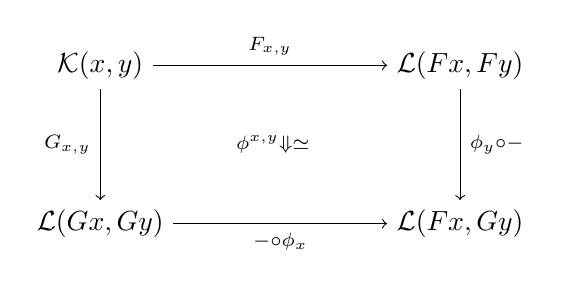
\begin{tikzpicture}[x=1.3em,y=1.3em]
  \node (tl) at (-4.2,2.2) {$\mathcal{K}(x,y)$};
  \node (tr) at (5.8,2.2) {$\mathcal{L}(Fx,Fy)$};
  \node (bl) at (-4.2,-2.2) {$\mathcal{L}(Gx,Gy)$};
  \node (br) at (5.8,-2.2) {$\mathcal{L}(Fx,Gy)$};
  \draw[->] (tl) -- node[above]{$\scriptstyle F_{x,y}$} (tr);
  \draw[->] (bl) -- node[below]{$\scriptstyle-\circ\phi_{x}$} (br);
  \draw[->] (tl) -- node[left]{$\scriptstyle G_{x,y}$} (bl);
  \draw[->] (tr) -- node[right]{$\scriptstyle\phi_{y}\circ-$} (br);
  \node at (0.6,0) {$\scriptstyle\phi^{x,y}\Downarrow\simeq$};
\end{tikzpicture}
\end{center}
\end{itemize}
使得这批数据尊重由诸拟伪函子指定的复合约束与单位约束，如下面两幅粘贴图所示：

\begin{center}
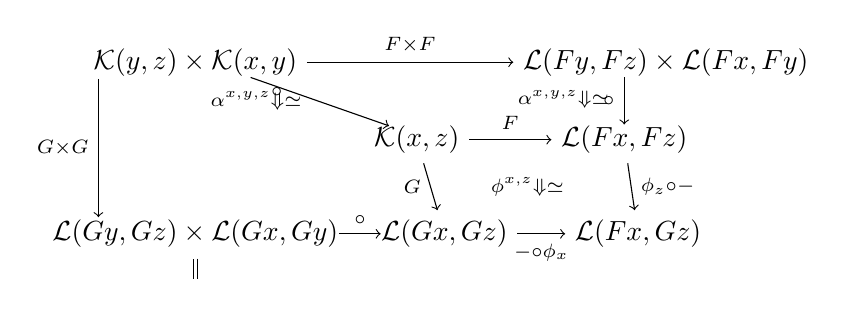
\begin{tikzpicture}[x=1em,y=1em]
  \node (A) at (0,0) {$\mathcal{K}(y,z)\times\mathcal{K}(x,y)$};
  \node (B) at (17,0) {$\mathcal{L}(Fy,Fz)\times\mathcal{L}(Fx,Fy)$};
  \node (C) at (8,-2.8) {$\mathcal{K}(x,z)$};
  \node (D) at (15.5,-2.8) {$\mathcal{L}(Fx,Fz)$};
  \node (E) at (0,-6.2) {$\mathcal{L}(Gy,Gz)\times\mathcal{L}(Gx,Gy)$};
  \node (F) at (9,-6.2) {$\mathcal{L}(Gx,Gz)$};
  \node (G) at (16,-6.2) {$\mathcal{L}(Fx,Gz)$};
  \draw[->] (A) -- node[above]{$\scriptstyle F{\times}F$} (B);
  \draw[->] (2,-0.55) -- node[above,left,pos=0.3]{$\scriptstyle\circ$} (7,-2.3);
  \node at (2.2,-1.4) {$\scriptstyle\alpha^{x,y,z}\Downarrow\simeq$};
  \draw[->] (C) -- node[above]{$\scriptstyle F$} (D);
  \draw[->] (15.5,-0.55) -- node[left,pos=0.5]{$\scriptstyle\circ$} (15.5,-2.25);
  \draw[->] (-3.5,-0.6) -- node[left]{$\scriptstyle G{\times}G$} (-3.5,-5.6);
  \node at (13.3,-1.35) {$\scriptstyle\alpha^{x,y,z}\Downarrow\simeq$};
  \draw[->] (C) -- node[left]{$\scriptstyle G$} (F);
  \draw[->] (D) -- node[right]{$\scriptstyle\phi_{z}\circ-$} (G);
  \node at (12,-4.5) {$\scriptstyle\phi^{x,z}\Downarrow\simeq$};
  \draw[->] (5.2,-6.2) -- node[above]{$\scriptstyle\circ$} (6.7,-6.2);
  \draw[->] (F) -- node[below]{$\scriptstyle-\circ\phi_{x}$} (G);
  \draw[double,double distance=1.2pt] (0,-7.1) -- (0,-7.85);
\end{tikzpicture}
\par\vspace{0.4em}
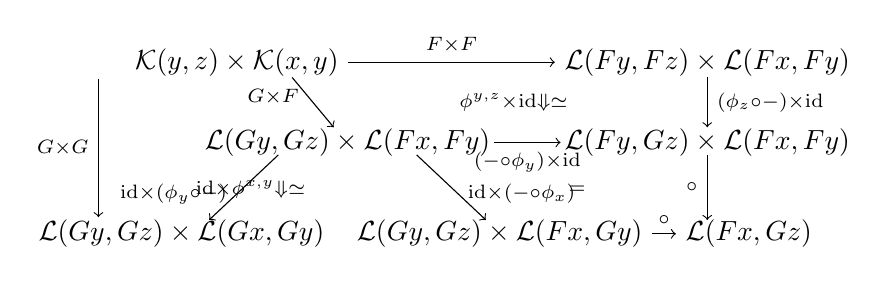
\begin{tikzpicture}[x=1em,y=1em]
  \node (A) at (0,0) {$\mathcal{K}(y,z)\times\mathcal{K}(x,y)$};
  \node (B) at (17,0) {$\mathcal{L}(Fy,Fz)\times\mathcal{L}(Fx,Fy)$};
  \node (M1) at (4,-2.9) {$\mathcal{L}(Gy,Gz)\times\mathcal{L}(Fx,Fy)$};
  \node (M2) at (17,-2.9) {$\mathcal{L}(Fy,Gz)\times\mathcal{L}(Fx,Fy)$};
  \node (E) at (-2,-6.2) {$\mathcal{L}(Gy,Gz)\times\mathcal{L}(Gx,Gy)$};
  \node (N) at (9.5,-6.2) {$\mathcal{L}(Gy,Gz)\times\mathcal{L}(Fx,Gy)$};
  \node (R) at (18.5,-6.2) {$\mathcal{L}(Fx,Gz)$};
  \draw[->] (A) -- node[above]{$\scriptstyle F{\times}F$} (B);
  \draw[->] (2,-0.55) -- node[left,pos=0.4]{$\scriptstyle G{\times}F$} (3.5,-2.35);
  \node at (10,-1.45) {$\scriptstyle\phi^{y,z}{\times}\mathrm{id}\Downarrow\simeq$};
  \draw[->] (17,-0.55) -- node[right,pos=0.5]{$\scriptstyle(\phi_{z}\circ-){\times}\mathrm{id}$} (17,-2.35);
  \draw[->] (9.3,-2.9) -- node[below]{$\scriptstyle(-\circ\phi_{y}){\times}\mathrm{id}$} (11.7,-2.9);
  \draw[->] (-5,-0.6) -- node[left]{$\scriptstyle G{\times}G$} (-5,-5.6);
  \draw[->] (1.5,-3.35) -- node[left,pos=0.6]{$\scriptstyle\mathrm{id}{\times}(\phi_{y}\circ-)$} (-1,-5.7);
  \node at (0.5,-4.6) {$\scriptstyle\mathrm{id}{\times}\phi^{x,y}\Downarrow\simeq$};
  \draw[->] (6.5,-3.35) -- node[right,pos=0.6]{$\scriptstyle\mathrm{id}{\times}(-\circ\phi_{x})$} (9,-5.7);
  \node at (12.3,-4.6) {$\scriptstyle=$};
  \draw[->] (17,-3.35) -- node[left,pos=0.5]{$\scriptstyle\circ$} (17,-5.7);
  \draw[->] (N) -- node[above]{$\scriptstyle\circ$} (R);
\end{tikzpicture}
\end{center}
\par 以及
\begin{center}
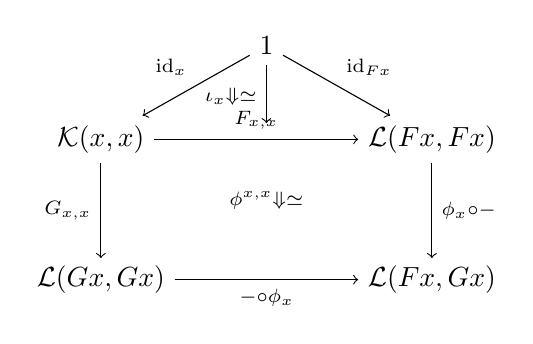
\begin{tikzpicture}[x=1.3em,y=1.3em]
  \node (1u) at (0,4.4) {$\mathbb{1}$};
  \node (tl) at (-4.6,1.8) {$\mathcal{K}(x,x)$};
  \node (tr) at (4.6,1.8) {$\mathcal{L}(Fx,Fx)$};
  \draw[->] (1u) -- node[above left]{$\scriptstyle\mathrm{id}_{x}$} (tl);
  \draw[->] (1u) -- node[above right]{$\scriptstyle\mathrm{id}_{Fx}$} (tr);
  \draw[->] (1u) -- node[left,pos=0.55]{$\scriptstyle\iota_{x}\Downarrow\simeq$} (0,2.25);
  \draw[->] (tl) -- node[above]{$\scriptstyle F_{x,x}$} (tr);
  \draw[->] (tl) -- node[left]{$\scriptstyle G_{x,x}$} (-4.6,-1.5);
  \draw[->] (tr) -- node[right]{$\scriptstyle\phi_{x}\circ-$} (4.6,-1.5);
  \node at (0,0.1) {$\scriptstyle\phi^{x,x}\Downarrow\simeq$};
  \node (bl) at (-4.6,-2.1) {$\mathcal{L}(Gx,Gx)$};
  \node (br) at (4.6,-2.1) {$\mathcal{L}(Fx,Gx)$};
  \draw[->] (bl) -- node[below]{$\scriptstyle-\circ\phi_{x}$} (br);
\end{tikzpicture}
\quad$=$\quad
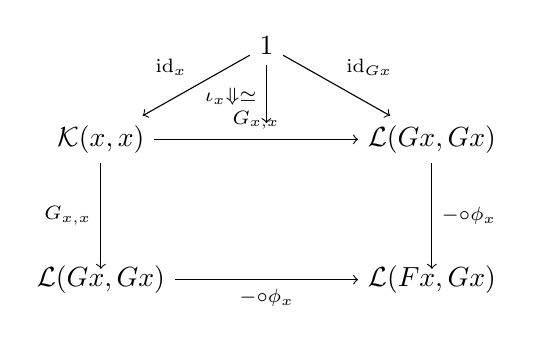
\begin{tikzpicture}[x=1.3em,y=1.3em]
  \node (1u) at (0,4.4) {$\mathbb{1}$};
  \node (tl) at (-4.6,1.8) {$\mathcal{K}(x,x)$};
  \node (tr) at (4.6,1.8) {$\mathcal{L}(Gx,Gx)$};
  \draw[->] (1u) -- node[above left]{$\scriptstyle\mathrm{id}_{x}$} (tl);
  \draw[->] (1u) -- node[above right]{$\scriptstyle\mathrm{id}_{Gx}$} (tr);
  \draw[->] (1u) -- node[left,pos=0.55]{$\scriptstyle\iota_{x}\Downarrow\simeq$} (0,2.25);
  \draw[->] (tl) -- node[above]{$\scriptstyle G_{x,x}$} (tr);
  \draw[->] (tl) -- node[left]{$\scriptstyle G_{x,x}$} (-4.6,-1.8);
  \draw[->] (tr) -- node[right]{$\scriptstyle-\circ\phi_{x}$} (4.6,-1.8);
  \node (bl) at (-4.6,-2.1) {$\mathcal{L}(Gx,Gx)$};
  \node (br) at (4.6,-2.1) {$\mathcal{L}(Fx,Gx)$};
  \draw[->] (bl) -- node[below]{$\scriptstyle-\circ\phi_{x}$} (br);
\end{tikzpicture}
\end{center}
\footnote{左图之中部 2-胞腔原书印作「$\phi^{x,y}\Downarrow\simeq$」，然图中仅涉
对象 $x$，应为 $\phi^{x,x}$ 之误，此处径改。——译者注}
\end{definition}

\begin{remark}\label{rem:analogy-pseudonatural-quasi}
定义 10.4.2 与定义 10.4.10 之间的类似性，平行于定义 10.4.1 与定义 10.4.4 之间的
类似性——只是这层类似被我们的陈述方式遮蔽了。伪函子 $F$、$G\colon\mathcal{C}\rightsquigarrow\mathcal{D}$
之间的伪自然变换 $\phi\colon F\Rrightarrow G$ 之可逆 2-\trCell{}分量的自然性要求告诉我们：
它们可以装配成\trFunctor{}之间的一个自然同构
\begin{center}
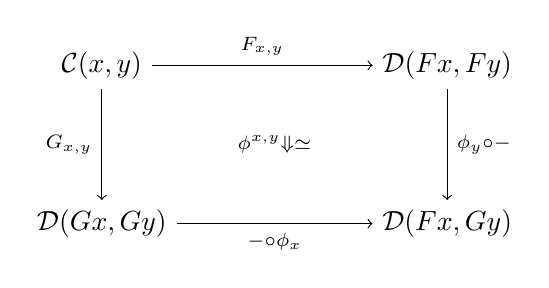
\begin{tikzpicture}[x=1.3em,y=1.3em]
  \node (tl) at (-4.2,2.2) {$\mathcal{C}(x,y)$};
  \node (tr) at (5.4,2.2) {$\mathcal{D}(Fx,Fy)$};
  \node (bl) at (-4.2,-2.2) {$\mathcal{D}(Gx,Gy)$};
  \node (br) at (5.4,-2.2) {$\mathcal{D}(Fx,Gy)$};
  \draw[->] (tl) -- node[above]{$\scriptstyle F_{x,y}$} (tr);
  \draw[->] (bl) -- node[below]{$\scriptstyle-\circ\phi_{x}$} (br);
  \draw[->] (tl) -- node[left]{$\scriptstyle G_{x,y}$} (bl);
  \draw[->] (tr) -- node[right]{$\scriptstyle\phi_{y}\circ-$} (br);
  \node at (0.6,0) {$\scriptstyle\phi^{x,y}\Downarrow\simeq$};
\end{tikzpicture}
\end{center}
对每一对 $x$、$y\in\mathcal{C}$ 成立。表达这些自然同构与复合约束及单位约束相容的
诸相干条件，随后可以写成定义 10.4.10 中出现的那种形式；但由于两个自然同构相等，
当且仅当它们的分量相等，我们可以把这些相干条件化归为定义 10.4.2 的其余两条粘贴
等式——用 $\phi$ 的分量表出。

\trQuasiCategory{}之间的\trFunctor{}之间的自然同构，其数据比\trCategory{}之间的\trFunctor{}之间
的自然同构更为错综；这正是定义 10.4.10 的诸相干条件必须以更普遍的方式表出的原因。不过，定义 10.4.2 的诸相干条件可以从这些条件中如下抽取出来。

请回忆：$\mathcal{K}(x,y)$ 中的 0-箭头对应于\trFunctor{}
$f\colon\mathbb{1}\to\mathcal{K}(x,y)$。由\cref{rem:terminal-qcat-notation}，限制
$\phi^{x,y}f$ 定义了 $\mathfrak{h}\mathcal{L}$ 中一个可逆 2-\trCell{}的分量
\begin{center}
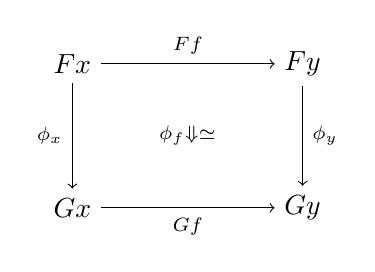
\begin{tikzpicture}[x=1.3em,y=1.3em]
  \node (tl) at (-3.2,2) {$Fx$};
  \node (tr) at (3.2,2) {$Fy$};
  \node (bl) at (-3.2,-2) {$Gx$};
  \node (br) at (3.2,-2) {$Gy$};
  \draw[->] (tl) -- node[above]{$\scriptstyle Ff$} (tr);
  \draw[->] (bl) -- node[below]{$\scriptstyle Gf$} (br);
  \draw[->] (tl) -- node[left]{$\scriptstyle\phi_{x}$} (bl);
  \draw[->] (tr) -- node[right]{$\scriptstyle\phi_{y}$} (br);
  \node at (0,0) {$\scriptstyle\phi_{f}\Downarrow\simeq$};
\end{tikzpicture}
\end{center}
这一 2-\trCell{}自动是自然的，其意义为：对 $\mathcal{K}$ 的\trHomotopyTwoCategory{}中的
每个 2-\trCell{}
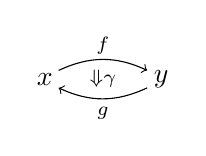
\begin{tikzpicture}[x=1em,y=0.9em,baseline=-0.5em]
  \node (x) at (0,0) {$x$};
  \node (y) at (4.2,0) {$y$};
  \draw[->] (0.5,0.35) to[bend left=25] (3.7,0.35);
  \node at (2.1,1.35) {$\scriptstyle f$};
  \draw[->] (3.7,-0.35) to[bend left=25] (0.5,-0.35);
  \node at (2.1,-1.35) {$\scriptstyle g$};
  \node at (2.1,0) {$\scriptstyle\Downarrow\gamma$};
\end{tikzpicture}，
粘贴复合
\begin{center}
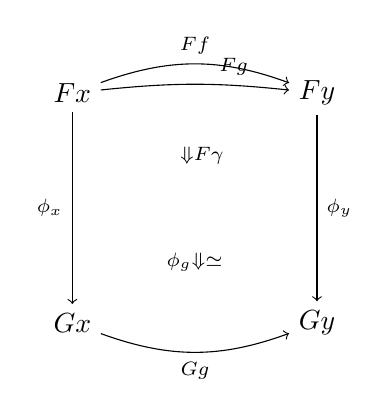
\begin{tikzpicture}[x=1.3em,y=1.3em]
  \node (tl) at (-3.4,3.2) {$Fx$};
  \node (tr) at (3.4,3.2) {$Fy$};
  \node (bl) at (-3.4,-3.2) {$Gx$};
  \node (br) at (3.4,-3.2) {$Gy$};
  \draw[->] (tl) to[bend left=20] node[above]{$\scriptstyle Ff$} (tr);
  \draw[->] (tl) to[bend left=6] node[above,pos=0.72]{$\scriptstyle Fg$} (tr);
  \node at (0.2,1.45) {$\scriptstyle\Downarrow F\gamma$};
  \draw[->] (tl) -- node[left]{$\scriptstyle\phi_{x}$} (bl);
  \draw[->] (tr) -- node[right]{$\scriptstyle\phi_{y}$} (br);
  \node at (0,-1.5) {$\scriptstyle\phi_{g}\Downarrow\simeq$};
  \draw[->] (bl) to[bend right=20] node[below]{$\scriptstyle Gg$} (br);
\end{tikzpicture}
\quad$=$\quad
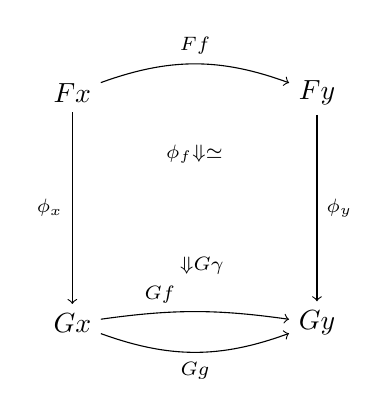
\begin{tikzpicture}[x=1.3em,y=1.3em]
  \node (tl) at (-3.4,3.2) {$Fx$};
  \node (tr) at (3.4,3.2) {$Fy$};
  \node (bl) at (-3.4,-3.2) {$Gx$};
  \node (br) at (3.4,-3.2) {$Gy$};
  \draw[->] (tl) to[bend left=20] node[above]{$\scriptstyle Ff$} (tr);
  \node at (0,1.5) {$\scriptstyle\phi_{f}\Downarrow\simeq$};
  \draw[->] (tl) -- node[left]{$\scriptstyle\phi_{x}$} (bl);
  \draw[->] (tr) -- node[right]{$\scriptstyle\phi_{y}$} (br);
  \draw[->] (bl) to[bend left=8] node[above,pos=0.3]{$\scriptstyle Gf$} (br);
  \node at (0.2,-1.6) {$\scriptstyle\Downarrow G\gamma$};
  \draw[->] (bl) to[bend right=20] node[below]{$\scriptstyle Gg$} (br);
\end{tikzpicture}
\end{center}
在 $\mathcal{L}$ 的\trHomotopyTwoCategory{}中相等。这由须状复合的自然性（见附录 B 中的%
\cref{lem:naturality-of-whiskering}）
得出，因为两个粘贴复合都由诸\trQuasiCategory{}的\trHomotopyTwoCategory{}中的如下水平复合
\begin{center}
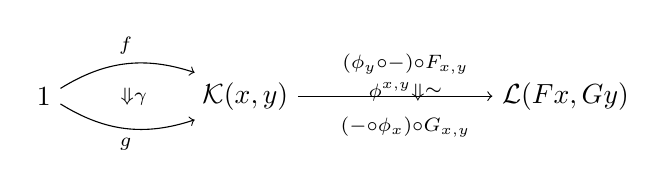
\begin{tikzpicture}[x=1.3em,y=1.3em]
  \node (1u) at (0,0) {$\mathbb{1}$};
  \node (K) at (5.6,0) {$\mathcal{K}(x,y)$};
  \node (L) at (14.5,0) {$\mathcal{L}(Fx,Gy)$};
  \draw[->] (1u) to[bend left=25] node[above]{$\scriptstyle f$} (K);
  \draw[->] (1u) to[bend right=25] node[below]{$\scriptstyle g$} (K);
  \node at (2.5,0) {$\scriptstyle\Downarrow\gamma$};
  \draw[->] (K) -- (L);
  \node at (10.05,0.9) {$\scriptstyle(\phi_{y}\circ-)\circ F_{x,y}$};
  \node at (10.05,0.12) {$\scriptstyle\phi^{x,y}\Downarrow\simeq$};
  \node at (10.05,-0.85) {$\scriptstyle(-\circ\phi_{x})\circ G_{x,y}$};
\end{tikzpicture}
\end{center}
所表示。

类似地，定义 10.4.10 的复合图表与单位图表蕴含：定义 10.4.2 中所展示的相应图表在
$\mathcal{L}$ 的\trHomotopyTwoCategory{}中交换（见\cref{ex:pasting-equalities-quasi}）。
\end{remark}

对任意拟范畴富集\trCategory{} $\mathcal{K}$，hom-\trBifunctor{}
$\mathcal{K}(-,-)\colon\mathcal{K}^{\mathrm{op}}\times\mathcal{K}\to\QCat{}$ 是一个
拟范畴富集\trFunctor。

\begin{lemma}\label{lem:action-on-homs-qpn}
拟伪函子 $F\colon\mathcal{K}\rightsquigarrow\mathcal{L}$（介于诸拟范畴富集%
\trCategory{} $\mathcal{K}$ 与 $\mathcal{L}$ 之间）在 hom 上的作用，定义了一个拟伪
自然变换
\begin{equation*}
F_{-,-}\colon\mathcal{K}(-,-)\Rrightarrow\mathcal{L}(F-,F-)
\end{equation*}
介于拟伪自然函子 $\mathcal{K}^{\mathrm{op}}\times\mathcal{K}\rightsquigarrow\QCat{}$
之间。
\footnote{此处「拟伪自然函子」照录原书面貌（quasi-pseudonatural
functors）；按上下文（前段已证 $\mathcal{K}(-,-)$ 为拟范畴富集\trFunctor）疑为
「拟范畴富集函子」（quasi-categorically enriched functors）之误。——译者注}
\end{lemma}

\begin{proof}
与 $\mathcal{K}^{\mathrm{op}}\times\mathcal{K}$ 中一对对象 $(x,y)$ 与 $(w,z)$ 相关联
的该拟伪自然变换之 2-\trCell{}分量为
\begin{center}
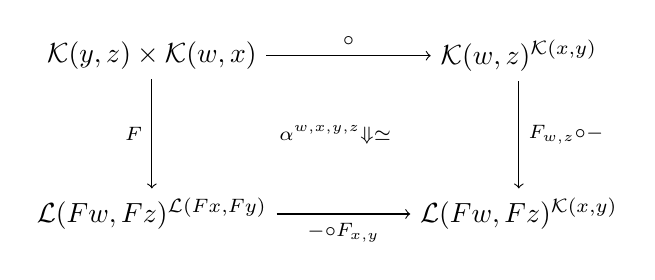
\begin{tikzpicture}[x=1.3em,y=1.3em]
  \node (tl) at (-4.6,2.2) {$\mathcal{K}(y,z)\times\mathcal{K}(w,x)$};
  \node (tr) at (5.6,2.2) {$\mathcal{K}(w,z)^{\mathcal{K}(x,y)}$};
  \node (bl) at (-4.6,-2.2) {$\mathcal{L}(Fw,Fz)^{\mathcal{L}(Fx,Fy)}$};
  \node (br) at (5.6,-2.2) {$\mathcal{L}(Fw,Fz)^{\mathcal{K}(x,y)}$};
  \draw[->] (tl) -- node[above]{$\scriptstyle\circ$} (tr);
  \draw[->] (bl) -- node[below]{$\scriptstyle-\circ F_{x,y}$} (br);
  \draw[->] (tl) -- node[left]{$\scriptstyle F$} (bl);
  \draw[->] (tr) -- node[right]{$\scriptstyle F_{w,z}\circ-$} (br);
  \node at (0.5,0) {$\scriptstyle\alpha^{w,x,y,z}\Downarrow\simeq$};
\end{tikzpicture}
\end{center}
其中 $\alpha^{w,x,y,z}$ 是 \eqref{eq:quasi-pseudofunctor-pasting} 所定义的公共
2-\trCell{}的一个转置。复合公理与单位公理的验证留给\cref{ex:finish-lemma-proof}。
\end{proof}

\begin{definition}\label{def:quasi-pseudonatural-equivalence}
余定义域为一个\trInfinityCosmos{}的、拟伪函子 $F$、$G\colon\mathcal{K}\rightsquigarrow\mathcal{L}$
之间的拟伪自然变换 $\phi\colon F\Rrightarrow G$，若其每个分量
$\phi_{x}\colon Fx\to Gx$ 都定义 $\mathcal{L}$ 的\trHomotopyTwoCategory{}中的一个%
\trEquivalence，便是一个\textbf{拟伪自然等价}。
\end{definition}

由于\cref{rem:quasi-biequivalence-cosmos-codomain}中所述的理由，假定 $\mathcal{L}$
是一个\trInfinityCosmos{}是方便的，这样我们便无须对目标\trCategory{}中\trEquivalence{}的
恰当概念作进一步的明确。我们对拟伪自然等价这一类的兴趣源于下述结果——它可以理解
为\trBicategory{} \trYonedaLemma{}在拟范畴富集\trCategory、拟伪函子与拟伪自然变换之语境中的
一个版本。

\begin{lemma}\label{lem:quasi-yoneda}
若在\trInfinityCosmos{} $\mathcal{K}$ 中由一对对象 $a$、$b$ 所\trRepresentable{}%
诸\trSimplicialFunctor{} $\mathcal{K}^{\mathrm{op}}\to\QCat{}$ 之间存在一条拟伪自然
等价
\begin{equation*}
\phi\colon\mathcal{K}(-,a)\Rrightarrow\mathcal{K}(-,b)
\end{equation*}
则 $a$ 与 $b$ 在 $\mathcal{K}$ 中等价。
\end{lemma}

\begin{proof}
我们将证明：0-箭头 $y\coloneqq\phi_{a}(\mathrm{id}_{a})\colon a\to b$ 是 $\mathcal{K}$
中的一个\trEquivalence。首先观察到：对每个 $x\in\mathcal{K}$，分量
$\phi_{x}\colon\mathcal{K}(x,a)\Rightarrow\mathcal{K}(x,b)$——下图中的右上复合——
在诸\trQuasiCategory{}的\trHomotopyTwoCategory{}中同构于经 $y$ 的后复合——即
下图中的左下复合：
\begin{center}
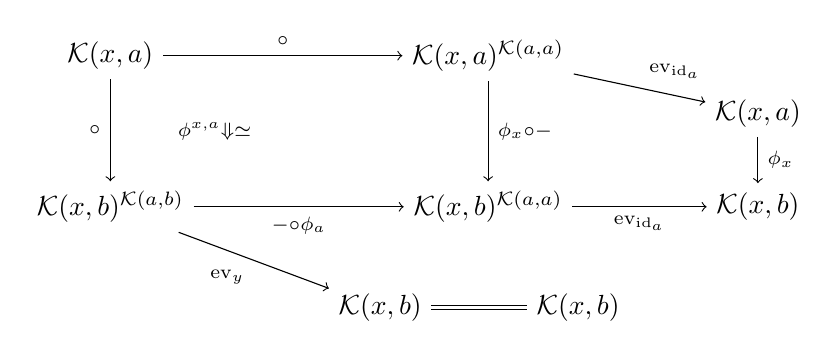
\begin{tikzpicture}[x=1.3em,y=1.3em]
  \node (P1) at (0,0) {$\mathcal{K}(x,a)$};
  \node (P2) at (10.5,0) {$\mathcal{K}(x,a)^{\mathcal{K}(a,a)}$};
  \node (P3) at (0,-4.2) {$\mathcal{K}(x,b)^{\mathcal{K}(a,b)}$};
  \node (P4) at (10.5,-4.2) {$\mathcal{K}(x,b)^{\mathcal{K}(a,a)}$};
  \node (P5) at (18,-1.6) {$\mathcal{K}(x,a)$};
  \node (P6) at (18,-4.2) {$\mathcal{K}(x,b)$};
  \node (P7) at (7.5,-7) {$\mathcal{K}(x,b)$};
  \node (P8) at (13,-7) {$\mathcal{K}(x,b)$};
  \draw[->] (P1) -- node[above]{$\scriptstyle\circ$} (P2);
  \draw[->] (P1) -- node[left]{$\scriptstyle\circ$} (P3);
  \node at (2.9,-2.1) {$\scriptstyle\phi^{x,a}\Downarrow\simeq$};
  \draw[->] (P2) -- node[right]{$\scriptstyle\phi_{x}\circ-$} (P4);
  \draw[->] (P3) -- node[below]{$\scriptstyle-\circ\phi_{a}$} (P4);
  \draw[->] (P4) -- node[below]{$\scriptstyle\mathrm{ev}_{\mathrm{id}_{a}}$} (P6);
  \draw[->] (P2) -- node[above right]{$\scriptstyle\mathrm{ev}_{\mathrm{id}_{a}}$} (P5);
  \draw[->] (P5) -- node[right]{$\scriptstyle\phi_{x}$} (P6);
  \draw[->] (P3) -- node[below left]{$\scriptstyle\mathrm{ev}_{y}$} (P7);
  \draw[double,double distance=1.2pt] (P7) -- (P8);
\end{tikzpicture}
\quad$\eqqcolon$\quad
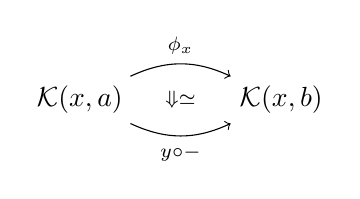
\begin{tikzpicture}[x=1.3em,y=1.3em]
  \node (l) at (0,0) {$\mathcal{K}(x,a)$};
  \node (r) at (5.6,0) {$\mathcal{K}(x,b)$};
  \draw[->] (l) to[bend left=25] node[above]{$\scriptstyle\phi_{x}$} (r);
  \draw[->] (l) to[bend right=25] node[below]{$\scriptstyle y\circ-$} (r);
  \node at (2.8,0) {$\scriptstyle\Downarrow\simeq$};
\end{tikzpicture}
\end{center}
特别地，由练习 1.4.iii，映射 $y\circ-\colon\mathcal{K}(x,a)\Rightarrow\mathcal{K}(x,b)$
对任何 $x\in\mathcal{K}$ 都是一个\trEquivalence，这意味着
$y\colon a\Rightarrow b$ 是\trInfinityCosmos{} $\mathcal{K}$ 中的一个%
\trEquivalence。
\end{proof}

拟伪自然等价可以构造为：逐分量定义\trEquivalence{}的那些\trSimplicial{}自然变换之
伴随等价逆。

\begin{lemma}\label{lem:adjoint-inverses-qpn}
考虑∞-宇宙间的拟范畴富集\trFunctor{}间的\trSimplicial{}自然变换
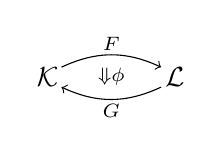
\begin{tikzpicture}[x=1em,y=0.9em,baseline=-0.5em]
  \node (K) at (0,0) {$\mathcal{K}$};
  \node (L) at (4.6,0) {$\mathcal{L}$};
  \draw[->] (0.5,0.4) to[bend left=25] (4.1,0.4);
  \node at (2.3,1.35) {$\scriptstyle F$};
  \node at (2.3,0) {$\scriptstyle\Downarrow\phi$};
  \draw[->] (4.1,-0.4) to[bend left=25] (0.5,-0.4);
  \node at (2.3,-1.35) {$\scriptstyle G$};
\end{tikzpicture}，
其中 0-箭头分量 $\phi_{x}\colon Fx\Rightarrow Gx$ 全都定义 $\mathcal{L}$ 中的%
\trEquivalence。则伴随等价逆 $\psi_{x}\colon Gx\Rightarrow Fx$ 的任何选取都可装配成一条
拟伪自然变换 $\psi\colon G\Rrightarrow F$ 的诸分量，后者是一个拟伪自然等价。
\end{lemma}

\begin{proof}
拟伪自然变换 $\psi$ 的诸分量由伴随等价逆箭头 $\psi_{x}\colon Gx\Rightarrow Fx$ 与下述粘贴
复合自然变换定义
\begin{center}
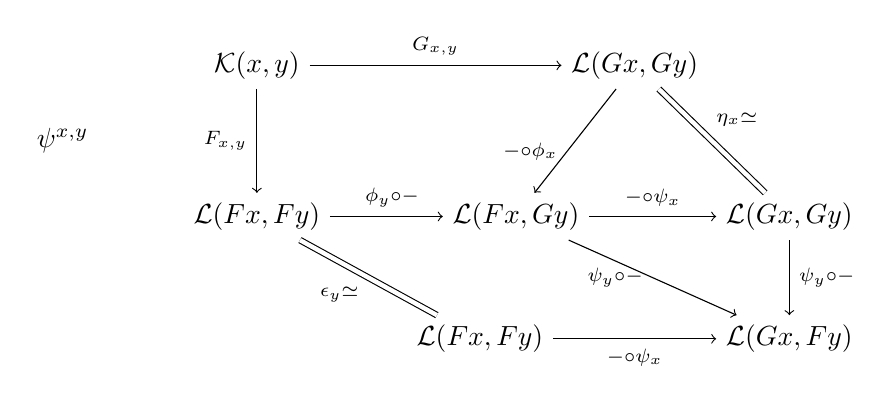
\begin{tikzpicture}[x=1.3em,y=1.3em]
  \node (Q1) at (0,0) {$\mathcal{K}(x,y)$};
  \node (Q2) at (10.5,0) {$\mathcal{L}(Gx,Gy)$};
  \node (Q3) at (0,-4.2) {$\mathcal{L}(Fx,Fy)$};
  \node (Q4) at (7.2,-4.2) {$\mathcal{L}(Fx,Gy)$};
  \node (Q5) at (14.8,-4.2) {$\mathcal{L}(Gx,Gy)$};
  \node (Q6) at (6.2,-7.6) {$\mathcal{L}(Fx,Fy)$};
  \node (Q7) at (14.8,-7.6) {$\mathcal{L}(Gx,Fy)$};
  \node at (-5.4,-2.1) {$\psi^{x,y}\coloneqq$};
  \draw[->] (Q1) -- node[above]{$\scriptstyle G_{x,y}$} (Q2);
  \draw[->] (Q1) -- node[left]{$\scriptstyle F_{x,y}$} (Q3);
  \draw[->] (Q2) -- node[left,pos=0.6]{$\scriptstyle-\circ\phi_{x}$} (Q4);
  \draw[double,double distance=1.6pt] (Q2) -- node[above right,pos=0.45]{$\scriptstyle\eta_{x}\simeq$} (Q5);
  \draw[->] (Q3) -- node[above,pos=0.55]{$\scriptstyle\phi_{y}\circ-$} (Q4);
  \draw[->] (Q4) -- node[above]{$\scriptstyle-\circ\psi_{x}$} (Q5);
  \draw[->] (Q4) -- node[left,pos=0.5]{$\scriptstyle\psi_{y}\circ-$} (Q7);
  \draw[->] (Q5) -- node[right]{$\scriptstyle\psi_{y}\circ-$} (Q7);
  \draw[double,double distance=1.6pt] (Q3) -- node[below left,pos=0.5]{$\scriptstyle\epsilon_{y}\simeq$} (Q6);
  \draw[->] (Q6) -- node[below]{$\scriptstyle-\circ\psi_{x}$} (Q7);
\end{tikzpicture}
\end{center}
涉及该伴随等价的单位同构与余单位同构。

由于 $F$ 与 $G$ 是\trSimplicialFunctor，单位条件化简为只要求：这一粘贴自然变换在
恒同箭头 $\mathrm{id}_{x}\colon\mathbb{1}\to\mathcal{K}(x,x)$ 处的分量是一个恒同
2-\trCell{} $\mathrm{id}_{\psi_{x}}$。这一分量是粘贴复合
\begin{center}
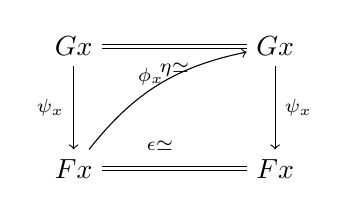
\begin{tikzpicture}[x=1.3em,y=1.3em]
  \node (A) at (-2.8,1.7) {$Gx$};
  \node (B) at (2.8,1.7) {$Gx$};
  \node (C) at (-2.8,-1.7) {$Fx$};
  \node (D) at (2.8,-1.7) {$Fx$};
  \draw[double,double distance=1.2pt] (A) -- (B);
  \draw[double,double distance=1.2pt] (C) -- (D);
  \draw[->] (A) -- node[left]{$\scriptstyle\psi_{x}$} (C);
  \draw[->] (B) -- node[right]{$\scriptstyle\psi_{x}$} (D);
  \draw[->] (C) to[bend left=20] node[left,pos=0.6]{$\scriptstyle\phi_{x}$} (B);
  \node at (0,1.05) {$\scriptstyle\eta\simeq$};
  \node at (-0.4,-1.05) {$\scriptstyle\epsilon\simeq$};
\end{tikzpicture}
\end{center}
由于所指定的数据定义一个伴随等价，这确为恒同。

类似地，为验证复合公理，我们必须证明复合
\begin{center}
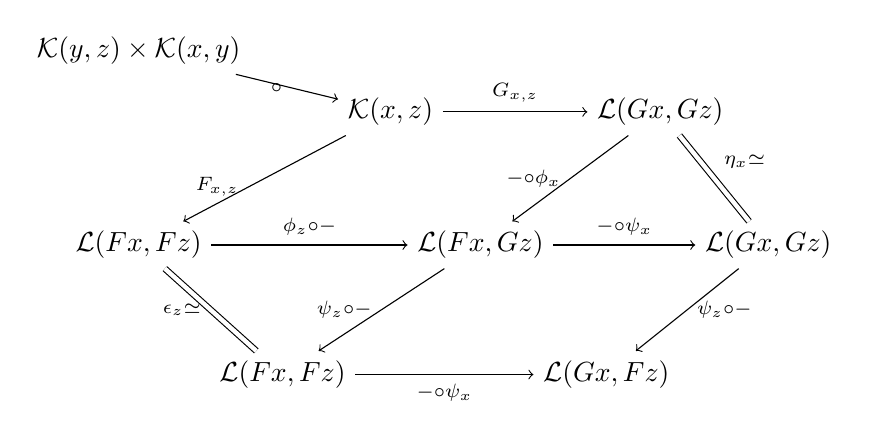
\begin{tikzpicture}[x=1.3em,y=1.3em]
  \node (V1) at (0,2) {$\mathcal{K}(y,z)\times\mathcal{K}(x,y)$};
  \node (V2) at (7,0.3) {$\mathcal{K}(x,z)$};
  \node (V3) at (14.5,0.3) {$\mathcal{L}(Gx,Gz)$};
  \node (V4) at (0,-3.4) {$\mathcal{L}(Fx,Fz)$};
  \node (V5) at (9.5,-3.4) {$\mathcal{L}(Fx,Gz)$};
  \node (V6) at (17.5,-3.4) {$\mathcal{L}(Gx,Gz)$};
  \node (V7) at (4,-7) {$\mathcal{L}(Fx,Fz)$};
  \node (V8) at (13,-7) {$\mathcal{L}(Gx,Fz)$};
  \draw[->] (V1) -- node[above,left,pos=0.55]{$\scriptstyle\circ$} (V2);
  \draw[->] (V2) -- node[above]{$\scriptstyle G_{x,z}$} (V3);
  \draw[->] (V2) -- node[left,pos=0.6]{$\scriptstyle F_{x,z}$} (V4);
  \draw[->] (V3) -- node[left]{$\scriptstyle-\circ\phi_{x}$} (V5);
  \draw[double,double distance=1.6pt] (V3) -- node[above right,pos=0.5]{$\scriptstyle\eta_{x}\simeq$} (V6);
  \draw[->] (V4) -- node[above]{$\scriptstyle\phi_{z}\circ-$} (V5);
  \draw[->] (V5) -- node[above]{$\scriptstyle-\circ\psi_{x}$} (V6);
  \draw[double,double distance=1.6pt] (V4) -- node[left,pos=0.5]{$\scriptstyle\epsilon_{z}\simeq$} (V7);
  \draw[->] (V5) -- node[left]{$\scriptstyle\psi_{z}\circ-$} (V7);
  \draw[->] (V6) -- node[right]{$\scriptstyle\psi_{z}\circ-$} (V8);
  \draw[->] (V7) -- node[below]{$\scriptstyle-\circ\psi_{x}$} (V8);
\end{tikzpicture}
\end{center}
等于
\begin{center}
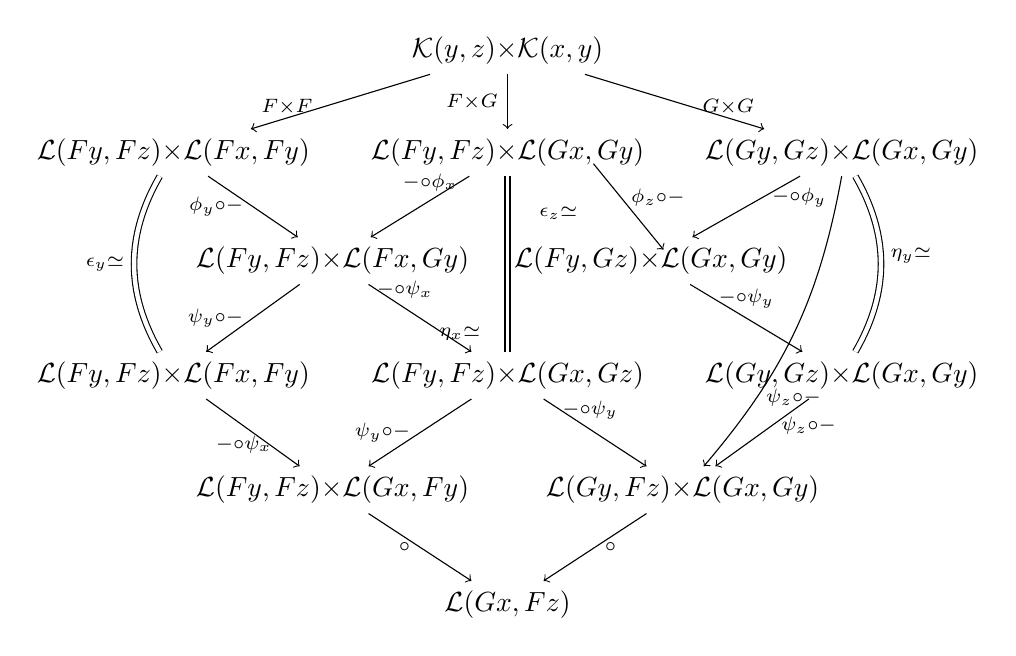
\begin{tikzpicture}[x=1.15em,y=1.15em]
  \node (K) at (10.5,0) {$\mathcal{K}(y,z){\times}\mathcal{K}(x,y)$};
  \node (L2) at (0,-3.2) {$\mathcal{L}(Fy,Fz){\times}\mathcal{L}(Fx,Fy)$};
  \node (M2) at (10.5,-3.2) {$\mathcal{L}(Fy,Fz){\times}\mathcal{L}(Gx,Gy)$};
  \node (R2) at (21,-3.2) {$\mathcal{L}(Gy,Gz){\times}\mathcal{L}(Gx,Gy)$};
  \node (L3) at (5,-6.6) {$\mathcal{L}(Fy,Fz){\times}\mathcal{L}(Fx,Gy)$};
  \node (M3) at (15,-6.6) {$\mathcal{L}(Fy,Gz){\times}\mathcal{L}(Gx,Gy)$};
  \node (L4) at (0,-10.2) {$\mathcal{L}(Fy,Fz){\times}\mathcal{L}(Fx,Fy)$};
  \node (M4) at (10.5,-10.2) {$\mathcal{L}(Fy,Fz){\times}\mathcal{L}(Gx,Gz)$};
  \node (L5) at (5,-13.8) {$\mathcal{L}(Fy,Fz){\times}\mathcal{L}(Gx,Fy)$};
  \node (R5) at (16,-13.8) {$\mathcal{L}(Gy,Fz){\times}\mathcal{L}(Gx,Gy)$};
  \node (R2p) at (21,-10.2) {$\mathcal{L}(Gy,Gz){\times}\mathcal{L}(Gx,Gy)$};
  \node (Z) at (10.5,-17.4) {$\mathcal{L}(Gx,Fz)$};
  \draw[->] (K) -- node[above,left,pos=0.6]{$\scriptstyle F{\times}F$} (L2);
  \draw[->] (K) -- node[left]{$\scriptstyle F{\times}G$} (M2);
  \draw[->] (K) -- node[above,right,pos=0.6]{$\scriptstyle G{\times}G$} (R2);
  \draw[->] (L2) -- node[left,pos=0.5]{$\scriptstyle\phi_{y}\circ-$} (L3);
  \draw[->] (M2) -- node[above,pos=0.4]{$\scriptstyle-\circ\phi_{x}$} (L3);
  \draw[->] (13.2,-3.55) -- node[right,pos=0.4]{$\scriptstyle\phi_{z}\circ-$} (15.4,-6.25);
  \draw[double,double distance=1.4pt] (M2) -- (M4);
  \node at (12.1,-5.1) {$\scriptstyle\epsilon_{z}\simeq$};
  \node at (9.0,-8.9) {$\scriptstyle\eta_{x}\simeq$};
  \draw[->] (R2) -- node[right,pos=0.35]{$\scriptstyle-\circ\phi_{y}$} (M3);
  \draw[->] (L3) -- node[left]{$\scriptstyle\psi_{y}\circ-$} (L4);
  \draw[->] (L3) -- node[above,pos=0.35]{$\scriptstyle-\circ\psi_{x}$} (M4);
  \draw[->] (M3) -- node[above,pos=0.5]{$\scriptstyle-\circ\psi_{y}$} (R2p);
  \draw[double,double distance=1.6pt] (L2) to[bend right=30] node[left,pos=0.5]{$\scriptstyle\epsilon_{y}\simeq$} (L4);
  \draw[double,double distance=1.6pt] (R2) to[bend left=30] node[right,pos=0.45]{$\scriptstyle\eta_{y}\simeq$} (R2p);
  \draw[->] (L4) -- node[below,pos=0.4]{$\scriptstyle-\circ\psi_{x}$} (L5);
  \draw[->] (M4) -- node[left,pos=0.5]{$\scriptstyle\psi_{y}\circ-$} (L5);
  \draw[->] (M4) -- node[above,pos=0.45]{$\scriptstyle-\circ\psi_{y}$} (R5);
  \draw[->] (R2.south) to[bend left=15] node[right,pos=0.75]{$\scriptstyle\psi_{z}\circ-$} (R5);
  \draw[->] (R2p) -- node[right,pos=0.4]{$\scriptstyle\psi_{z}\circ-$} (R5);
  \draw[->] (L5) -- node[above,left]{$\scriptstyle\circ$} (Z);
  \draw[->] (R5) -- node[above,right]{$\scriptstyle\circ$} (Z);
\end{tikzpicture}
\end{center}
图中出现的\trPreComposition{}映射与\trPostComposition{}映射都是 2-自然的（见定义 B.2.2），因此例如
$\epsilon_{y}$ 与 $-\circ\psi_{x}$ 的须状复合可以按任意一次序构成。在第二幅粘贴图
中反复使用这条交换性质，并运用三角等式
$\phi_{y}\epsilon_{y}\cdot\eta_{y}\phi_{y}=\mathrm{id}_{\phi_{y}}$，第二幅粘贴图便
化归为第一幅。
\end{proof}

现在我们证明：诸\trInfinityCosmos{}之间的任何一支\trBiequivalence{}
$F\colon\mathcal{K}\Rightarrow\mathcal{L}$ 都容许一个拟伪函子性的「逆」
$G\colon\mathcal{L}\rightsquigarrow\mathcal{K}$，并配备拟伪自然等价
$\eta\colon\mathrm{id}_{\mathcal{K}}\Rrightarrow GF$ 与
$\epsilon\colon FG\Rrightarrow\mathrm{id}_{\mathcal{L}}$。

\begin{proposition}\label{prop:quasi-pseudoinverse}
若 $F\colon\mathcal{K}\to\mathcal{L}$ 是诸\trInfinityCosmos{}之间的一个拟范畴
富集\trFunctor{}兼\trBiequivalence，则存在一个拟伪函子
$G\colon\mathcal{L}\rightsquigarrow\mathcal{K}$，它也是一支\trBiequivalence。而且，
$G$ 是 $F$ 的一个\emph{拟伪逆}，其意义为：存在拟伪自然等价
$\mathrm{id}_{\mathcal{K}}\Rrightarrow GF$ 与 $FG\Rrightarrow\mathrm{id}_{\mathcal{L}}$。
\end{proposition}

\begin{proof}
为融贯地定义\trBiequivalence{} $F\colon\mathcal{K}\Rightarrow\mathcal{L}$ 的一支逆，
我们「完整指定」其数据，选取：
\begin{itemize}
\item[($\beta$)] 对每个 $a\in\mathcal{L}$，完整指定的伴随等价
$\epsilon_{a}\colon Fx_{a}\simeq a$；并且
\item[($\gamma$)] 对每一对 $x$、$y\in\mathcal{K}$，完整指定的、诸拟范畴之伴随等价的逆
\begin{equation*}
\mathcal{K}(x,y)\xrightarrow[\ \sim\ ]{F_{x,y}}\mathcal{L}(Fx,Fy)
\end{equation*}
其逆对 $x$ 与 $y$ 是拟伪自然的。
\end{itemize}
在 ($\gamma$) 中，我们将\cref{lem:adjoint-inverses-qpn}应用于\trSimplicial{}自然变换
$F_{-,-}\colon\mathcal{K}(-,-)\to\mathcal{L}(F-,F-)$，从而观察到：对这些映射逐点取的
伴随等价可装配成一个拟伪自然变换，而且后者还是一个逐点等价。
\footnote{原书印作「In $(\gamma)$, we apply to the simplicial natural
transformation $F_{-,-}\colon\mathcal{K}(-,-)\to\mathcal{L}(F-,F-)$ to
observe…」，apply 之后疑脱漏所引条目名；按文义（伴随等价逆装配成拟伪自然变换）
应为引理 10.4.15，据文义补。——译者注}

现在，为定义 $G\colon\mathcal{L}\rightsquigarrow\mathcal{K}$，用 ($\beta$) 为每个
$a\in\mathcal{L}$ 指定一个对象 $Ga\coloneqq x_{a}\in\mathcal{K}$，连同一支\trEquivalence{}
$\epsilon_{a}\colon FGa\simeq a$（在 $\mathcal{L}$ 中）。这就定义了 $G$ 在对象上的
映射以及拟伪自然变换 $\epsilon$ 的 0-箭头分量。为定义 $G$ 在诸\trFunctorSpace{}上的
作用，用这批数据与 ($\gamma$) 定义
\begin{equation*}
G_{a,b}\coloneqq\mathcal{L}(a,b)
\xrightarrow[\ \sim\ ]{\ (-\circ\epsilon_{a},\,\epsilon_{b}^{-1}\circ-)\ }
\mathcal{L}(FGa,FGb)
\xrightarrow[\ \sim\ ]{\ F_{Ga,Gb}^{-1}\ }
\mathcal{K}(Ga,Gb)
\end{equation*}

对每个 $a\in\mathcal{L}$，定义 $\iota_{a}\colon\mathrm{id}_{Ga}\cong G_{a,a}\,\mathrm{id}_{a}$
为下述复合
\begin{center}
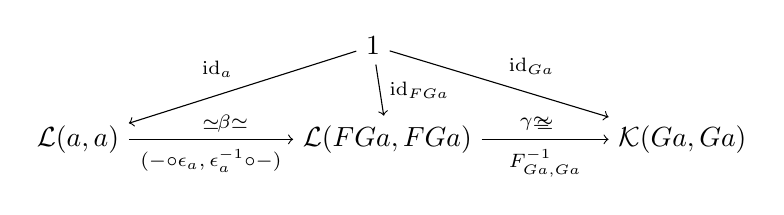
\begin{tikzpicture}[x=1.3em,y=1.3em]
  \node (1u) at (0,2.6) {$\mathbb{1}$};
  \node (l) at (-8.2,0) {$\mathcal{L}(a,a)$};
  \node (m) at (0.4,0) {$\mathcal{L}(FGa,FGa)$};
  \node (r) at (8.6,0) {$\mathcal{K}(Ga,Ga)$};
  \draw[->] (1u) -- node[above left]{$\scriptstyle\mathrm{id}_{a}$} (l);
  \draw[->] (1u) -- node[above right]{$\scriptstyle\mathrm{id}_{Ga}$} (r);
  \draw[->] (1u) -- node[right,pos=0.5]{$\scriptstyle\mathrm{id}_{FGa}$} (m);
  \node at (-3.9,0.45) {$\scriptstyle\beta\simeq$};
  \node at (4.5,0.45) {$\scriptstyle\gamma\simeq$};
  \draw[->] (l) -- node[above]{$\scriptstyle\simeq$}
    node[below]{$\scriptstyle(-\circ\epsilon_{a},\,\epsilon_{a}^{-1}\circ-)$} (m);
  \draw[->] (m) -- node[above]{$\scriptstyle\simeq$}
    node[below]{$\scriptstyle F_{Ga,Ga}^{-1}$} (r);
\end{tikzpicture}
\end{center}
即把 $\mathfrak{h}\mathcal{L}$ 中的\trIsomorphism{}
$\beta_{a}\colon\epsilon_{a}^{-1}\circ\epsilon_{a}\cong\mathrm{id}_{FGa}$ 与%
\trIsomorphism{}
$\gamma\colon F_{Ga,Ga}^{-1}\circ F_{Ga,Ga}\cong\mathrm{id}_{\mathcal{K}(Ga,Ga)}$ 在
$\mathrm{id}_{Ga}$ 处的分量。对每个 $a$、$b$、$c\in\mathcal{L}$，定义 $\alpha^{a,b,c}$
为由 ($\beta$) 与 ($\gamma$) 之数据构造的诸典范\trNaturalTransformation{}的如下复合
\begin{center}
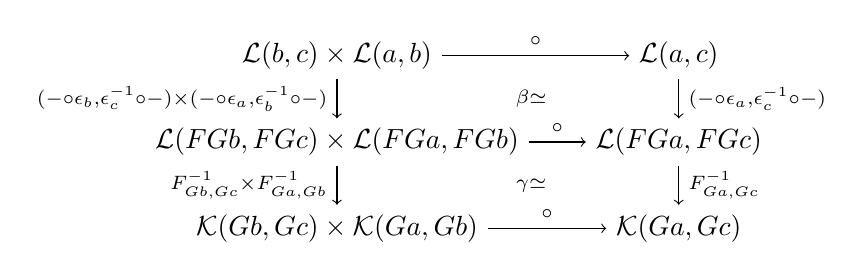
\begin{tikzpicture}[x=1.3em,y=1.3em]
  \node (W1) at (0,2.4) {$\mathcal{L}(b,c)\times\mathcal{L}(a,b)$};
  \node (W2) at (9.5,2.4) {$\mathcal{L}(a,c)$};
  \node (X1) at (0,0) {$\mathcal{L}(FGb,FGc)\times\mathcal{L}(FGa,FGb)$};
  \node (X2) at (9.5,0) {$\mathcal{L}(FGa,FGc)$};
  \node (Y1) at (0,-2.4) {$\mathcal{K}(Gb,Gc)\times\mathcal{K}(Ga,Gb)$};
  \node (Y2) at (9.5,-2.4) {$\mathcal{K}(Ga,Gc)$};
  \draw[->] (W1) -- node[above]{$\scriptstyle\circ$} (W2);
  \draw[->] (X1) -- node[above]{$\scriptstyle\circ$} (X2);
  \draw[->] (Y1) -- node[above]{$\scriptstyle\circ$} (Y2);
  \draw[->] (W1) -- node[left]{$\scriptstyle(-\circ\epsilon_{b},\epsilon_{c}^{-1}\circ-)\times(-\circ\epsilon_{a},\epsilon_{b}^{-1}\circ-)$} (X1);
  \draw[->] (W2) -- node[right]{$\scriptstyle(-\circ\epsilon_{a},\epsilon_{c}^{-1}\circ-)$} (X2);
  \node at (5.4,1.2) {$\scriptstyle\beta\simeq$};
  \draw[->] (X1) -- node[left]{$\scriptstyle F_{Gb,Gc}^{-1}{\times}F_{Ga,Gb}^{-1}$} (Y1);
  \draw[->] (X2) -- node[right]{$\scriptstyle F_{Ga,Gc}^{-1}$} (Y2);
  \node at (5.4,-1.2) {$\scriptstyle\gamma\simeq$};
\end{tikzpicture}
\end{center}

我们接着验证：这些选取使 $G$ 成为一个拟伪函子。为单位条件，我们必须验证复合
\begin{center}
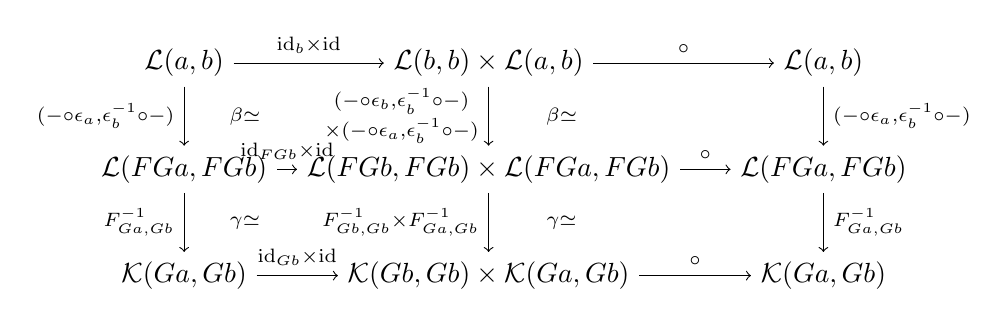
\begin{tikzpicture}[x=1.1em,y=1.6em]
  \node (U11) at (0,2.4) {$\mathcal{L}(a,b)$};
  \node (U12) at (10,2.4) {$\mathcal{L}(b,b)\times\mathcal{L}(a,b)$};
  \node (U13) at (21,2.4) {$\mathcal{L}(a,b)$};
  \node (U21) at (0,0) {$\mathcal{L}(FGa,FGb)$};
  \node (U22) at (10,0) {$\mathcal{L}(FGb,FGb)\times\mathcal{L}(FGa,FGb)$};
  \node (U23) at (21,0) {$\mathcal{L}(FGa,FGb)$};
  \node (U31) at (0,-2.4) {$\mathcal{K}(Ga,Gb)$};
  \node (U32) at (10,-2.4) {$\mathcal{K}(Gb,Gb)\times\mathcal{K}(Ga,Gb)$};
  \node (U33) at (21,-2.4) {$\mathcal{K}(Ga,Gb)$};
  \draw[->] (U11) -- node[above]{$\scriptstyle\mathrm{id}_{b}{\times}\mathrm{id}$} (U12);
  \draw[->] (U12) -- node[above]{$\scriptstyle\circ$} (U13);
  \draw[->] (U21) -- node[above]{$\scriptstyle\mathrm{id}_{FGb}{\times}\mathrm{id}$} (U22);
  \draw[->] (U22) -- node[above]{$\scriptstyle\circ$} (U23);
  \draw[->] (U31) -- node[above]{$\scriptstyle\mathrm{id}_{Gb}{\times}\mathrm{id}$} (U32);
  \draw[->] (U32) -- node[above]{$\scriptstyle\circ$} (U33);
  \draw[->] (U11) -- node[left]{$\scriptstyle(-\circ\epsilon_{a},\epsilon_{b}^{-1}\circ-)$} (U21);
  \node at (2.0,1.2) {$\scriptstyle\beta\simeq$};
  \draw[->] (U12) -- node[left,align=center]{$\scriptstyle(-\circ\epsilon_{b},\epsilon_{b}^{-1}\circ-)$\\[-0.3ex]$\scriptstyle\times(-\circ\epsilon_{a},\epsilon_{b}^{-1}\circ-)$} (U22);
  \node at (12.4,1.2) {$\scriptstyle\beta\simeq$};
  \draw[->] (U13) -- node[right]{$\scriptstyle(-\circ\epsilon_{a},\epsilon_{b}^{-1}\circ-)$} (U23);
  \draw[->] (U21) -- node[left]{$\scriptstyle F_{Ga,Gb}^{-1}$} (U31);
  \node at (2.0,-1.2) {$\scriptstyle\gamma\simeq$};
  \draw[->] (U22) -- node[left]{$\scriptstyle F_{Gb,Gb}^{-1}{\times}F_{Ga,Gb}^{-1}$} (U32);
  \node at (12.4,-1.2) {$\scriptstyle\gamma\simeq$};
  \draw[->] (U23) -- node[right]{$\scriptstyle F_{Ga,Gb}^{-1}$} (U33);
\end{tikzpicture}
\end{center}
为恒同；事实上，每一对竖直复合都是恒同。在左手边，这得益于伴随等价 $\epsilon_{b}$
的三角等式关系之一；在右手边，这是\cref{lem:adjoint-inverses-qpn}所确立的
$F_{Ga,Gb}^{-1}$ 与 $\gamma$ 所成之偶的拟伪自然性的一个推论。右单位约束与结合性
条件与之类似。这就完成了「$G\colon\mathcal{L}\rightsquigarrow\mathcal{K}$ 定义一个
拟伪函子」的证明。

由构造，拟伪函子 $G$ 是一个\trLocalEquivalence：它在 hom 上的作用定义为一支%
\trEquivalence{}与一支映射之复合，而后者由在\trInfinityCosmos{} $\mathcal{L}$ 中与
诸\trEquivalence{}作\trPreComposition{}与\trPostComposition{}所诱导，于是由推论 1.4.8，它是一条\trEquivalence。
我们用这个\trLocalEquivalence{}来论证：对每个 $x\in\mathcal{K}$，存在一条\trEquivalence{}
$\eta_{x}\colon x\Rightarrow GFx$，从而证得 $G$ 的本质满性。这一分量定义为：把
($\gamma$) 中完整指定的逆伴随等价
$F_{x,GFx}^{-1}\colon\mathcal{L}(Fx,FGFx)\Rightarrow\mathcal{K}(x,GFx)$
应用到 ($\beta$) 中完整指定的伴随等价之逆 $\epsilon_{Fx}^{-1}\colon Fx\to FGFx$ 上。
由于 $F$ 是一支\trCosmologicalBiequivalence，它把映射 $\eta_{x}$ 携为 $\mathcal{L}$
中的一条\trEquivalence，故 $\eta_{x}$ 本身是 $\mathcal{K}$ 中的一条\trEquivalence。
这样，拟伪函子 $G$ 便是一支\trBiequivalence。

剩下的只是检验 $\eta$ 与 $\epsilon$ 的拟伪自然性。对后者，我们用如下粘贴图定义
分量自然同构
\begin{center}
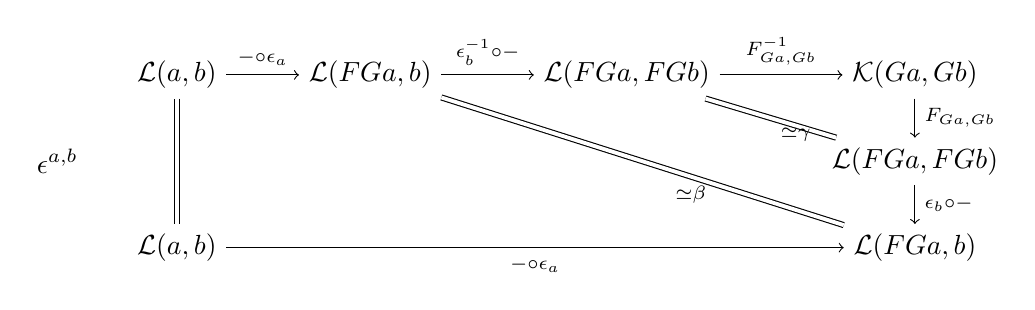
\begin{tikzpicture}[x=1.27em,y=1.3em]
  \node (E1) at (0,0) {$\mathcal{L}(a,b)$};
  \node (E2) at (5.5,0) {$\mathcal{L}(FGa,b)$};
  \node (E3) at (12.8,0) {$\mathcal{L}(FGa,FGb)$};
  \node (E4) at (21,0) {$\mathcal{K}(Ga,Gb)$};
  \node (E5) at (21,-2.4) {$\mathcal{L}(FGa,FGb)$};
  \node (E6) at (21,-4.8) {$\mathcal{L}(FGa,b)$};
  \node (E7) at (0,-4.8) {$\mathcal{L}(a,b)$};
  \node at (-3.4,-2.4) {$\epsilon^{a,b}\coloneqq$};
  \draw[->] (E1) -- node[above]{$\scriptstyle-\circ\epsilon_{a}$} (E2);
  \draw[->] (E2) -- node[above]{$\scriptstyle\epsilon_{b}^{-1}\circ-$} (E3);
  \draw[->] (E3) -- node[above]{$\scriptstyle F_{Ga,Gb}^{-1}$} (E4);
  \draw[->] (E4) -- node[right]{$\scriptstyle F_{Ga,Gb}$} (E5);
  \draw[double,double distance=1.4pt] (E3) -- node[below right,pos=0.5]{$\scriptstyle\simeq\gamma$} (E5);
  \draw[->] (E5) -- node[right]{$\scriptstyle\epsilon_{b}\circ-$} (E6);
  \draw[double,double distance=1.4pt] (E2) -- node[below,pos=0.62]{$\scriptstyle\simeq\beta$} (E6);
  \draw[double,double distance=1.4pt] (E1) -- (E7);
  \draw[->] (E7) -- node[below]{$\scriptstyle-\circ\epsilon_{a}$} (E6);
\end{tikzpicture}
\end{center}

对前者，利用定义 $\eta_{x}\coloneqq F^{-1}\epsilon_{Fx}^{-1}$ 与 $F_{-,-}$ 的拟伪
自然性，我们有粘贴图
\begin{center}
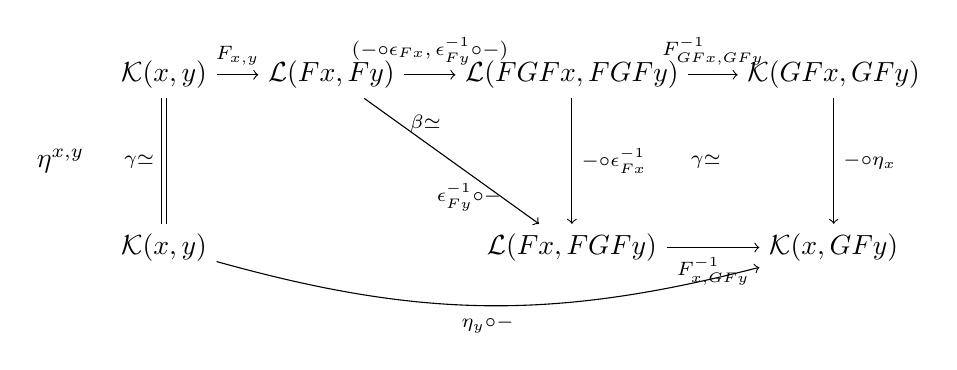
\begin{tikzpicture}[x=1.1em,y=1.3em]
  \node (H1) at (0,0) {$\mathcal{K}(x,y)$};
  \node (H2) at (5.5,0) {$\mathcal{L}(Fx,Fy)$};
  \node (H3) at (13.4,0) {$\mathcal{L}(FGFx,FGFy)$};
  \node (H4) at (22,0) {$\mathcal{K}(GFx,GFy)$};
  \node (H5) at (13.4,-4.8) {$\mathcal{L}(Fx,FGFy)$};
  \node (H6) at (22,-4.8) {$\mathcal{K}(x,GFy)$};
  \node (H7) at (0,-4.8) {$\mathcal{K}(x,y)$};
  \node at (-3.4,-2.4) {$\eta^{x,y}\coloneqq$};
  \draw[->] (H1) -- node[above]{$\scriptstyle F_{x,y}$} (H2);
  \draw[->] (H2) -- node[above]{$\scriptstyle(-\circ\epsilon_{Fx},\,\epsilon_{Fy}^{-1}\circ-)$} (H3);
  \draw[->] (H3) -- node[above]{$\scriptstyle F_{GFx,GFy}^{-1}$} (H4);
  \draw[->] (H2) -- node[above,pos=0.35]{$\scriptstyle\beta\simeq$}
    node[below,pos=0.6]{$\scriptstyle\epsilon_{Fy}^{-1}\circ-$} (H5);
  \draw[->] (H3) -- node[right]{$\scriptstyle-\circ\epsilon_{Fx}^{-1}$} (H5);
  \node at (17.8,-2.4) {$\scriptstyle\gamma\simeq$};
  \draw[->] (H4) -- node[right]{$\scriptstyle-\circ\eta_{x}$} (H6);
  \draw[->] (H5) -- node[below]{$\scriptstyle F_{x,GFy}^{-1}$} (H6);
  \draw[double,double distance=1.4pt] (H1) -- node[left]{$\scriptstyle\gamma\simeq$} (H7);
  \draw[->] (H7) to[bend right=15] node[below]{$\scriptstyle\eta_{y}\circ-$} (H6);
\end{tikzpicture}
\end{center}
它定义了分量的自然同构。这些自然变换为定义拟伪自然等价
$\eta\colon\mathrm{id}_{\mathcal{K}}\Rrightarrow GF$ 与
$\epsilon\colon FG\Rrightarrow\mathrm{id}_{\mathcal{L}}$ 而须满足的单位与复合相干
条件，其验证留给读者。
\end{proof}

由定义直接可得：拟伪函子之复合仍是拟伪函子，而\trBiequivalence{}之复合仍是%
\trBiequivalence。于是：

\begin{corollary}\label{cor:zigzag-quasi-pseudofunctor}
任何由\trCosmologicalBiequivalence{}构成的之字形链都复合而定义诸\trInfinityCosmos{}%
之间的一个拟伪函子 $\mathcal{K}\rightsquigarrow\mathcal{L}$，后者也是一支%
\trBiequivalence。
\end{corollary}

此外，命题 10.3.6 所确立的\trCosmologicalBiequivalence{}之保持性质与反射性质，可
推广到它们的拟伪函子性逆上——诚邀读者在\cref{ex:heuristic-reflection}中探究。

\subsection*{练习}

\begin{exercise}\label{ex:pseudofunctors-2-category}
对固定的一对 2-\trCategory{} $\mathcal{C}$ 与 $\mathcal{D}$，请证明：伪函子
$\mathcal{C}\rightsquigarrow\mathcal{D}$ 之搜集、其间的伪自然变换、以及这些之间的%
\trModification{}（见定义 B.2.3）可装配成一个 2-\trCategory。
\end{exercise}

\begin{exercise}\label{ex:pseudonatural-equivalence-characterization}
（[59, 6.2.16]）对 2-\trCategory{} $\mathcal{C}$ 与 $\mathcal{D}$ 之间的伪函子
$F$、$G\colon\mathcal{C}\rightsquigarrow\mathcal{D}$ 之间的一条伪自然变换
$\phi\colon F\Rrightarrow G$，请证明下述两条等价：
\begin{itemize}
\item 每个 1-\trCell{}分量 $\phi_{x}\colon Fx\Rightarrow Gx$ 是 $\mathcal{D}$ 中的一个%
\trEquivalence。
\item 1-\trCell{} $\phi$ 在\cref{ex:pseudofunctors-2-category}所描述的那座
2-\trCategory{}中定义一个\trEquivalence。
\end{itemize}
\end{exercise}

\begin{exercise}\label{ex:pasting-equalities-quasi}
设 $\phi\colon F\Rrightarrow G$ 为拟伪函子 $F$、$G\colon\mathcal{K}\rightsquigarrow\mathcal{L}$
之间的一条拟伪自然变换。对 $\mathcal{K}$ 中任意一对 0-箭头 $f\colon x\to y$ 与
$k\colon y\to z$，请在 $\mathcal{L}$ 的\trHomotopyTwoCategory{}中验证下列粘贴等式：
\begin{center}
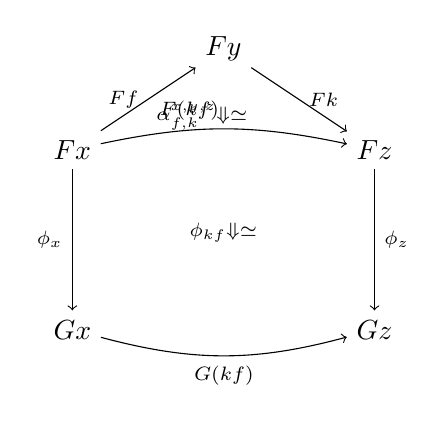
\begin{tikzpicture}[x=1.3em,y=1.3em]
  \node (fx) at (-4.2,0.6) {$Fx$};
  \node (fy) at (0,3.4) {$Fy$};
  \node (fz) at (4.2,0.6) {$Fz$};
  \node (gx) at (-4.2,-4.4) {$Gx$};
  \node (gz) at (4.2,-4.4) {$Gz$};
  \draw[->] (fx) -- node[above,left]{$\scriptstyle Ff$} (fy);
  \draw[->] (fy) -- node[above,right]{$\scriptstyle Fk$} (fz);
  \node at (-0.6,1.5) {$\scriptstyle\alpha^{x,y,z}_{f,k}\Downarrow\simeq$};
  \draw[->] (fx) to[bend left=12] node[above,pos=0.35]{$\scriptstyle F(kf)$} (fz);
  \node at (0,-1.7) {$\scriptstyle\phi_{kf}\Downarrow\simeq$};
  \draw[->] (fx) -- node[left]{$\scriptstyle\phi_{x}$} (gx);
  \draw[->] (fz) -- node[right]{$\scriptstyle\phi_{z}$} (gz);
  \draw[->] (gx) to[bend right=15] node[below]{$\scriptstyle G(kf)$} (gz);
\end{tikzpicture}
\quad$=$\quad
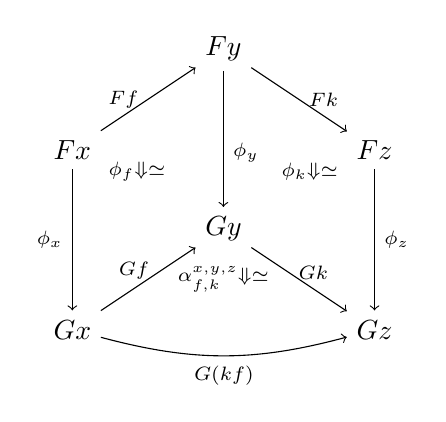
\begin{tikzpicture}[x=1.3em,y=1.3em]
  \node (fx) at (-4.2,0.6) {$Fx$};
  \node (fy) at (0,3.4) {$Fy$};
  \node (fz) at (4.2,0.6) {$Fz$};
  \node (gx) at (-4.2,-4.4) {$Gx$};
  \node (gy) at (0,-1.6) {$Gy$};
  \node (gz) at (4.2,-4.4) {$Gz$};
  \draw[->] (fx) -- node[above,left]{$\scriptstyle Ff$} (fy);
  \draw[->] (fy) -- node[above,right]{$\scriptstyle Fk$} (fz);
  \draw[->] (fx) -- node[left]{$\scriptstyle\phi_{x}$} (gx);
  \draw[->] (fy) -- node[right,pos=0.6]{$\scriptstyle\phi_{y}$} (gy);
  \draw[->] (fz) -- node[right]{$\scriptstyle\phi_{z}$} (gz);
  \node at (-2.4,0) {$\scriptstyle\phi_{f}\Downarrow\simeq$};
  \node at (2.4,0) {$\scriptstyle\phi_{k}\Downarrow\simeq$};
  \draw[->] (gx) -- node[above,pos=0.35]{$\scriptstyle Gf$} (gy);
  \draw[->] (gy) -- node[above,pos=0.65]{$\scriptstyle Gk$} (gz);
  \node at (0,-3.0) {$\scriptstyle\alpha^{x,y,z}_{f,k}\Downarrow\simeq$};
  \draw[->] (gx) to[bend right=15] node[below]{$\scriptstyle G(kf)$} (gz);
\end{tikzpicture}
\par 以及
\begin{tikzpicture}[x=1.3em,y=1.3em]
  \node (tl) at (-3.4,3.0) {$Fx$};
  \node (tr) at (3.4,3.0) {$Fx$};
  \node (bl) at (-3.4,-3.0) {$Gx$};
  \node (br) at (3.4,-3.0) {$Gx$};
  \draw[->] (tl) to[bend left=22] node[above]{$\scriptstyle\mathrm{id}_{Fx}$} (tr);
  \draw[->] (tl) to[bend left=8] node[above,pos=0.72]{$\scriptstyle F\,\mathrm{id}_{x}$} (tr);
  \node at (0,1.35) {$\scriptstyle\iota_{x}\Downarrow\simeq$};
  \draw[->] (tl) -- node[left]{$\scriptstyle\phi_{x}$} (bl);
  \draw[->] (tr) -- node[right]{$\scriptstyle\phi_{x}$} (br);
  \node at (0,-1.4) {$\scriptstyle\phi_{\mathrm{id}_{x}}\Downarrow\simeq$};
  \draw[->] (bl) to[bend right=22] node[below]{$\scriptstyle G\,\mathrm{id}_{x}$} (br);
\end{tikzpicture}
\quad$=$\quad
\begin{tikzpicture}[x=1.3em,y=1.3em]
  \node (tl) at (-3.4,3.0) {$Fx$};
  \node (tr) at (3.4,3.0) {$Fx$};
  \node (bl) at (-3.4,-3.0) {$Gx$};
  \node (br) at (3.4,-3.0) {$Gx$};
  \draw[->] (tl) to[bend left=22] node[above]{$\scriptstyle\mathrm{id}_{Fx}$} (tr);
  \draw[->] (tl) -- node[left]{$\scriptstyle\phi_{x}$} (bl);
  \draw[->] (tr) -- node[right]{$\scriptstyle\phi_{x}$} (br);
  \draw[->] (bl) to[bend left=8] node[above,pos=0.28]{$\scriptstyle\mathrm{id}_{Gx}$} (br);
  \node at (0,-1.35) {$\scriptstyle\iota_{x}\Downarrow\simeq$};
  \draw[->] (bl) to[bend right=22] node[below]{$\scriptstyle G\,\mathrm{id}_{x}$} (br);
\end{tikzpicture}
\end{center}
\footnote{右下图之中部 2-胞腔原书亦印作「$\iota_{y}\Downarrow\simeq$」，同定义
10.4.2 单位约束图处之勘注，径改。——译者注}
\end{exercise}

\begin{exercise}\label{ex:finish-lemma-proof}
请完成\cref{lem:action-on-homs-qpn}的证明。
\end{exercise}

\begin{exercise}\label{ex:derive-prop-1043}
从\cref{prop:quasi-pseudoinverse}之证明出发，按\cref{rem:quasi-biequivalence-cosmos-codomain}
作修改，导出\cref{prop:pseudoinverse-2-functor}的一个证明。
\end{exercise}

\begin{exercise}\label{ex:heuristic-reflection}
请发展一个启发性论证，解释为何凡由一支\trCosmologicalBiequivalence{}保持并反射的
∞-范畴论性质或结构，也都由其逆拟伪函子保持并反射。
\end{exercise}













